%%%%%%%%%%%%%%%%%%%%%%%%%%%%%%%%%%%%%%%%%%%%%%%%%%%%%%%%%%%%%%%%%%%%%%%%%%%%%%%%%%%%%%%%%
% Khóa luận tốt nghiệp/Tiểu luận 
% LaTeX Template
% Phiên bản 1.0 (tạo ra ngày 05/10/2022)
%
% Template này có thể được download tại:
% https://github.com/cpc1996/HUS-Dissertation-Template
%
% Phiên bản 1.0 được chỉnh sửa bởi:
% Công Phương Cao (congphuongcao@gmail.com)
% Nguyễn Cảnh Việt (vietncp@gmail.com)
%
% Template được tham khảo từ một phiên bản template của:
% Steve Gunn (http://users.ecs.soton.ac.uk/srg/softwaretools/document/templates/)
% Sunil Patel (http://www.sunilpatel.co.uk/thesis-template/)
%
%%%%%%%%%%%%%%%%%%%%%%%%%%%%%%%%%%%%%%%%%%%%%%%%%%%%%%%%%%%%%%%%%%%%%%%%%%%%%%%%%%%%%%%%%


%----------------------------------------------------------------------------------------
%	(KHÔNG CHỈNH SỬA PHẦN NÀY)
%
%	PHẦN 1: CÁC PACKAGE CƠ BẢN VÀ CÁC TÙY CHỈNH VĂN BẢN
%----------------------------------------------------------------------------------------

\documentclass[
12pt,
oneside,
english,
doublespacing,
nolistspacing,
liststotoc,
parskip,
headsepline,
chapterinoneline,
]{HUSdissertation}

% \usepackage[utf8]{inputenc} 
\usepackage[utf8]{vietnam} 
%\usepackage[T1]{fontenc}

\usepackage{mathptmx}
\usepackage{amsmath}
\allowdisplaybreaks

%https://www.overleaf.com/learn/latex/Biblatex_citation_styles
%\usepackage[backend=bibtex,style=authoryear,natbib=true]{biblatex}
\usepackage[backend=bibtex,style=numeric,citestyle=ieee,natbib=true]{biblatex}

\addbibresource{main.bib}

\usepackage[autostyle=true]{csquotes}
\usepackage{float}

\usepackage[utf8]{inputenc}
\usepackage{babel} % <--- Đã xóa [vietnamese] để hết bị xung đột
\usepackage{tikz}
\usetikzlibrary{
    shapes.geometric,
    arrows.meta,
    positioning,
    shadows,
    calc
}
\usepackage{enumitem}
\usepackage{listings}
\usepackage{xcolor}

\lstset{
    language=Python,
    basicstyle=\ttfamily\small,
    keywordstyle=\color{blue},
    commentstyle=\color{green!50!black},
    stringstyle=\color{red},
    numbers=left,
    numberstyle=\tiny,
    breaklines=true,
    frame=single,
    showstringspaces=false,
    tabsize=4
}
%----------------------------------------------------------------------------------------
%	PHẦN 2: CÁC PACKAGE BỔ TRỢ THÊM VÀO TRONG QUÁ TRÌNH BIÊN SOẠN
%----------------------------------------------------------------------------------------

\RequirePackage{setlst}		% Liệt kê/trích dẫn code

\usepackage{multirow}
\usepackage{subfigure}
\usepackage[fontsize=13pt]{scrextend}

%https://www.sascha-frank.com/latex-font-size.html
%https://tex.stackexchange.com/questions/103286/how-to-change-section-subsection-font-size
\usepackage{titlesec}

\titleformat{\section}
{\normalfont\fontsize{13}{13}\bfseries}{\thesection}{1em}{}

\titleformat{\subsection}
{\normalfont\fontsize{13}{13}\bfseries\itshape}{\thesubsection}{1em}{}

%https://tex.stackexchange.com/questions/351961/how-to-indent-code-in-beginverbatim
\usepackage{fancyvrb} 		% Fancy Verbatim
\fvset{tabsize=4,vspace=0pt,fontsize=\footnotesize}

\usepackage{longtable} 		% Bảng dài - Long table

\usepackage[figuresright]{rotating} % Bảng ngang - Sideways table
\usepackage{tabularx}

\usepackage{fontawesome5} 	% Các biểu tượng, ký hiệu đặc biệt

\usepackage{tikz} 			% Vẽ hình
\usetikzlibrary{calc}

\usepackage{indentfirst}	% Lùi đầu dòng ở đầu đoạn văn
\setlength{\parindent}{0.5cm}

%----------------------------------------------------------------------------------------
%	PHẦN 3: THÔNG TIN VỀ Khóa luận tốt nghiệp/Tiểu luận (THESIS INFORMATION)
%----------------------------------------------------------------------------------------

\author{NHÓM 11} 			% Ví dụ: "Nguyễn Thị Thu Thảo"
\thesistitle{PHƯƠNG PHÁP NHẬN DIỆN VẬT CẢN VÀ ƯỚC LƯỢNG KHOẢNG CÁCH ĐỂ HỖ TRỢ NGƯỜI KHIẾM THỊ} % Ví dụ: "Nghiên cứu chế tạo và tính chất quang học của vật liệu nano LaF3:Sm3+"

\supervisor {TS. Nguyễn Tiến Cường} 	% Ví dụ: "PGS. TS. Nguyễn Ngọc Long"
\supervisorr{CN. Vi Anh Quân} 	% Tên này nếu không có thì để trống!

\field{Ngành Kỹ thuật Điện tử và Tin học} 					% Ví dụ: "Ngành Vật lý", "Ngành Hóa học", v.v.
\program{Chương trình đào tạo chuẩn} 			% Ví dụ: "Chương trình đào tạo chuẩn", "Chương trình đào tạo cử nhân tài năng", v.v.
\doctype{Đề tài môn Học Máy} % Điền vào đây: "Khóa luận tốt nghiệp đại học hệ chính quy" hoặc "Tiểu luận"

\university{\href{http://hus.vnu.edu.vn}{Trường Đại học Khoa học Tự nhiên}}
\department{\href{http://hus.vnu.edu.vn/gioi-thieu/co-cau-to-chuc/khoa-truc-thuoc/khoa-vat-ly.html}{Khoa Vật lý}}

\AtBeginDocument{
	\hypersetup{pdftitle=\ttitle}
	\hypersetup{pdfauthor=\authorname}
}


\begin{document}

\lstset{style=codeC}	% Thiết lập ngôn ngữ C/C++ là ngôn ngữ mặc định cho phần liệt kê souce code của cả bài

\frontmatter 			% Sử dụng hệ thống đánh số La Mã (i, ii, iii, iv...) cho những trang trước phần mục lục

\pagestyle{plain} 


%----------------------------------------------------------------------------------------
%	(KHÔNG CHỈNH SỬA PHẦN NÀY)
%
%	PHẦN 4: TRANG TIÊU ĐỀ/TRANG BÌA (TITLE PAGE)
%----------------------------------------------------------------------------------------

% TRANG BÌA CHÍNH:
\include{main-cover}

% TRANG BÌA PHỤ:
\include{sub-cover}


%----------------------------------------------------------------------------------------
%	PHẦN 5: DANH NGÔN (QUOTES)
%----------------------------------------------------------------------------------------

% \vspace*{0.2\textheight}

% \noindent\enquote{\itshape 
% 	Cái tôi và sự hiểu biết tỷ lệ nghịch với nhau. Hiểu biết càng nhiều cái tôi càng bé. Hiểu biết càng ít, cái tôi càng to.
% }\bigbreak

% \hfill Albert Einstein


%----------------------------------------------------------------------------------------
%	PHẦN 6: LỜI CẢM ƠN (ACKNOWLEDGEMENTS)
%----------------------------------------------------------------------------------------

\begin{acknowledgements}
	\addchaptertocentry{\acknowledgementname}
	\thispagestyle{empty}

Trong quá trình thực hiện môn học Học máy (Machine Learning) để hoàn thành bài báo cáo này, nhóm em đã nhận được sự hướng dẫn tận tình, sự quan tâm sâu sắc và những hỗ trợ quý báu từ thầy Nguyễn Tiến Cường và thầy Vi Anh Quân. Nhóm em xin gửi lời cảm ơn chân thành và sâu sắc đến các thầy vì đã luôn đồng hành, định hướng và hỗ trợ em trong suốt quá trình học tập cũng như triển khai đề tài. Trong suốt quá trình thực hiện, em đã được tiếp cận nhiều kiến thức quan trọng liên quan đến các mô hình học sâu, xử lý dữ liệu và ứng dụng trí tuệ nhân tạo trong thực tế. Những góp ý chuyên môn của các thầy không chỉ giúp em hoàn thiện nội dung bài báo cáo mà còn giúp em hiểu rõ hơn về tư duy giải quyết vấn đề trong lĩnh vực học máy.

Mặc dù đã cố gắng hoàn thiện bài báo cáo một cách tốt nhất trong khả năng của mình, nhưng do hạn chế về kiến thức và kinh nghiệm thực tiễn nên không thể tránh khỏi những thiếu sót. Nhóm em rất mong nhận được những ý kiến đóng góp, nhận xét và chỉ dẫn thêm từ các thầy để có thể tiếp tục hoàn thiện báo cáo trong thời gian tới.

Cuối cùng, nhóm em xin kính chúc thầy Nguyễn Tiến Cường và thầy Vi Anh Quân luôn mạnh khỏe, hạnh phúc và đạt được nhiều thành công trong sự nghiệp giảng dạy và nghiên cứu khoa học.

Nhóm em xin chân thành cảm ơn các thầy!
\end{acknowledgements}

\clearpage


\textbf{Nhóm sinh viên thực hiện}

\vspace{0.3cm}

\textbf{Lớp Kỹ thuật Điện tử và Tin học K68 -- Khoa Vật lý}

\vspace{0.5cm}

\begin{center}
\begin{tabular}{c l c}
\hline
\textbf{STT} & \textbf{Họ và tên -- Mã sinh viên} & \textbf{Tỷ lệ đóng góp (\%)} \\
\hline
1 & Nguyễn Tiến Dũng -- 23001585 & 40\\
2 & Hà Việt Anh -- 23001575 & 35\\
3 & Cao Văn Đạt -- 23001591 & 25\\
\hline
\end{tabular}
\end{center}

\clearpage
%----------------------------------------------------------------------------------------
%	(KHÔNG CHỈNH SỬA PHẦN NÀY)
%
%	PHẦN 7: MỤC LỤC (LIST OF CONTENTS/FIGURES/TABLES PAGES)
%----------------------------------------------------------------------------------------

\begin{spacing}{1.15}
	\tableofcontents 	% In ra mục lục chính
\end{spacing}

\begin{spacing}{1.15}
	\listoffigures 		% In ra danh sách hình vẽ
\end{spacing}

\begin{spacing}{1.15}
	\listoftables		% In ra danh sách bảng
\end{spacing}


%----------------------------------------------------------------------------------------
%	PHẦN 8: DANH SÁCH TÊN VIẾT TẮT (ABBREVIATIONS)
%----------------------------------------------------------------------------------------

\begin{abbreviations}{ll} % Thêm danh sách tên viết tắt (dưới dạng một bảng có 2 cột)

\textbf{AI} & Artificial Intelligence (Trí tuệ nhân tạo)\\
\textbf{YOLO} & You Only Look Once\\
\textbf{Faster R-CNN} & Faster Region-based Convolutional Neural Network\\
\textbf{RPN} & Region Proposal Network\\
\textbf{SSD} & Single Shot MultiBox Detector\\
\textbf{FPN} & Feature Pyramid Network\\
\textbf{PAN} & Path Aggregation Network\\
\textbf{RetinaNet} & Retina Network\\
\textbf{MiDaS} & Monocular Depth Estimation\\
\textbf{TTS} & Text-to-Speech\\
\textbf{CNN} & Convolutional Neural Network\\
\textbf{TAL} & Task-Aligned Learning\\
\textbf{NMS} & Non-Maximum Suppression\\
\textbf{DFL} & Distribution Focal Loss\\
\textbf{ONNX} & Open Neural Network Exchange\\
\textbf{STAL} & Small-Target-Aware Label Assignment\\
\textbf{SGD} & Stochastic Gradient Descent\\
\textbf{MuSGD} & Momentum-based Stochastic Gradient Descent\\
\textbf{MOT} & Multi-Object Tracking\\
\textbf{gTTS} & Google Text-to-Speech\\
\textbf{CLI} & Command Line Interface\\
\textbf{API} & Application Programming Interface\\
\textbf{HTTP} & HyperText Transfer Protocol\\
\textbf{NLP} & Natural Language Processing\\
\textbf{CPU} & Central Processing Unit\\
\textbf{CIoU} & Complete Intersection over Union\\
\textbf{IoU} & Intersection over Union\\
\textbf{MAE} & Mean Absolute Error\\
\textbf{MSE} & Mean Squared Error\\
\textbf{RMSE} & Root Mean Squared Error\\
\textbf{GPU} & Graphics Processing Unit\\
\textbf{MD5} & Message-Digest Algorithm 5\\

\end{abbreviations}


%----------------------------------------------------------------------------------------
%	PHẦN 9: CÁC HẰNG SỐ VẬT LÝ/THÔNG SỐ KĨ THUẬT (PHYSICAL CONSTANTS/OTHER DEFINITIONS)
%----------------------------------------------------------------------------------------

% \begin{constants}{lr@{${}={}$}l} % Thêm danh sách các hằng số (dưới dạng một bảng có 3 cột)

% %	Lệnh \SI{}{} được cung cấp bởi gói siunitx, hãy đọc tài liệu hướng dẫn để biết cách sử dụng nó

% %	Tên hằng số 	 & $Biểu tượng$	& $Hằng số$ cùng với đơn vị\\
% 	Vận tốc ánh sáng & $c_{0}$		& \SI{2.99792458e8}{\meter\per\second} (chính xác)\\

% \end{constants}


%----------------------------------------------------------------------------------------
%	PHẦN 10: DANH SÁCH KÝ HIỆU (SYMBOLS)
%----------------------------------------------------------------------------------------

% \begin{symbols}{lll} % Thêm danh sách các ký hiệu (dưới dạng một bảng có 3 cột)

% %   Ký hiệu	& Ý nghĩa		& Đơn vị \\
% 	$a$		& khoảng cách	& \si{\meter} \\
% 	$P$		& công suất		& \si{\watt} (\si{\joule\per\second}) \\

% 	\addlinespace % Khoảng cách để phân biệt giữa ký hiệu Latin với ký hiệu La Mã

% 	$\omega$ & tần số góc	& \si{\radian} \\

% \end{symbols}


%----------------------------------------------------------------------------------------
%	(KHÔNG CHỈNH SỬA PHẦN NÀY)
%
%	PHẦN 11: LỜI ĐỀ TẶNG (DEDICATION)
%----------------------------------------------------------------------------------------

%\dedicatory{Dành tặng/Dành cho/Gửi tới\ldots} 


%----------------------------------------------------------------------------------------
%	PHẦN 12: NỘI DUNG/CÁC CHƯƠNG Khóa luận tốt nghiệp/Tiểu luận (THESIS CONTENT - CHAPTERS)
%----------------------------------------------------------------------------------------

\mainmatter % Bắt đầu đánh số trang (1,2,3...)

\pagestyle{plain}

% Hãy thêm những chương (chapter) của khóa luận/tiểu luận vào thư mục Chapters
% Hãy bỏ chú thích những dòng nếu bạn đã bổ sung những chương vào

% MỞ ĐẦU (LỜI MỞ ĐẦU - Chương 0)

\chapter*{MỞ ĐẦU} % Tên của chương
\addcontentsline{toc}{chapter}{MỞ ĐẦU} % Thêm tên chương vào mục lục

\label{Chapter0} % Để trích dẫn chương này ở chỗ nào đó trong bài, hãy sử dụng lệnh \ref{Chapter0} 

%----------------------------------------------------------------------------------------

Trong bối cảnh công nghệ trí tuệ nhân tạo (AI) và thị giác máy tính đang phát triển
mạnh mẽ, các ứng dụng hỗ trợ con người trong đời sống ngày càng được quan tâm và
nghiên cứu rộng rãi. Đặc biệt, đối với người khiếm thị, việc di chuyển và nhận biết môi
trường xung quanh luôn là một thách thức lớn do hạn chế về khả năng quan sát. Những
khó khăn trong việc phát hiện vật cản, xác định khoảng cách hay nhận biết nguy hiểm
có thể ảnh hưởng trực tiếp đến sự an toàn và khả năng sinh hoạt độc lập của người
khiếm thị trong cuộc sống hằng ngày.

Hiện nay, nhiều giải pháp hỗ trợ người khiếm thị đã được nghiên cứu và phát triển,
từ các thiết bị cảm biến siêu âm truyền thống cho đến các hệ thống ứng dụng trí tuệ nhân
tạo và học sâu (Deep Learning). Trong đó, các phương pháp sử dụng thị giác máy tính
kết hợp với nhận diện đối tượng và ước lượng khoảng cách đang cho thấy nhiều tiềm
năng nhờ khả năng xử lý thông tin trực quan nhanh chóng, chính xác và có thể hoạt động
trong thời gian thực. Tuy nhiên, việc xây dựng các phương pháp có độ chính xác cao,
khả năng thích nghi tốt với môi trường thực tế và đáp ứng yêu cầu xử lý thời gian thực
vẫn còn là một bài toán cần được nghiên cứu và cải thiện.

Xuất phát từ thực tế đó, nhóm em lựa chọn đề tài “Phương pháp nhận diện vật cản và ước
lượng khoảng cách để hỗ trợ người khiếm thị”. Đề tài tập trung nghiên cứu các phương
pháp nhận diện vật cản dựa trên mô hình học sâu kết hợp với kỹ thuật ước lượng khoảng
cách nhằm hỗ trợ người khiếm thị trong quá trình di chuyển. Thông qua việc phân tích,
xây dựng và đánh giá các mô hình phù hợp, đề tài hướng tới việc nâng cao khả năng
nhận biết môi trường xung quanh, hỗ trợ cảnh báo vật cản và tăng độ an toàn cho người
khiếm thị.

Trong báo cáo này, nhóm em trình bày quá trình nghiên cứu lý thuyết, xây dựng phương
pháp, triển khai mô hình và đánh giá kết quả thực nghiệm cho bài toán nhận diện vật cản
và ước lượng khoảng cách nhằm hỗ trợ người khiếm thị. Báo cáo tập trung phân tích
cách thức hoạt động của mô hình, khả năng nhận diện vật cản cũng như hiệu quả ước
lượng khoảng cách trong các điều kiện thực tế khác nhau. Qua đó, đề tài hướng tới việc
đề xuất một phương pháp hỗ trợ người khiếm thị trong quá trình di chuyển, góp phần
nâng cao tính an toàn và khả năng ứng dụng của các giải pháp hỗ trợ thông minh trong
thực tế.
% Chương 1

\chapter{TỔNG QUAN ĐỀ TÀI} % Tên của chương

\label{Chapter1} % Để trích dẫn chương này ở chỗ nào đó trong bài, hãy sử dụng lệnh \ref{Chapter1} 

%----------------------------------------------------------------------------------------

% Định nghĩa một số lệnh cần thiết để điều chỉnh định dạng cho một số nội dung nhất định trong bài
\newcommand{\keyword}[1]{\textbf{#1}}
\newcommand{\tabhead}[1]{\textbf{#1}}
\newcommand{\code}[1]{\texttt{#1}}
\newcommand{\file}[1]{\texttt{\bfseries#1}}
\newcommand{\option}[1]{\texttt{\itshape#1}}

%----------------------------------------------------------------------------------------

\section{Giới thiệu bài toán}

Trong kỷ nguyên của trí tuệ nhân tạo và các hệ thống tự hành, bài toán nhận diện vật cản và ước lượng khoảng cách đã trở thành một trong những hướng nghiên cứu trọng tâm và tiên phong của lĩnh vực Thị giác máy tính (Computer Vision). Ý nghĩa của bài toán này không chỉ dừng lại ở việc tối ưu hóa công nghệ, mà còn mang giá trị nhân văn sâu sắc khi được ứng dụng để xây dựng các hệ thống điều hướng thông minh, hỗ trợ người khiếm thị tái hòa nhập cộng đồng. Đối với người khiếm thị, việc di chuyển trong môi trường thực tế là một thách thức lớn khi xung quanh luôn tồn tại các mối nguy cơ chuyển động liên tục và bất ngờ như người đi bộ, xe máy, ô tô, hoặc các chướng ngại vật tĩnh như cột điện, biển báo, bàn ghế. Một hệ thống trợ thính hoặc trợ thị thông minh không chỉ cần đóng vai trò như một đôi mắt thứ hai để nhận biết môi trường, mà còn phải là một bộ não có khả năng phân tích không gian trong thời gian thực, từ đó đưa ra những chỉ dẫn an toàn và kịp thời cho người dùng.

Để giải quyết trọn vẹn bài toán hỗ trợ điều hướng, hệ thống không thể dựa vào một kỹ thuật đơn lẻ mà phải phối hợp nhịp nhàng một chuỗi các tác vụ phức tạp theo trình tự tuyến tính. Đầu tiên là tác vụ nhận diện đối tượng (Object Detection) nhằm phân tích các khung hình thu nhận từ camera để xác định chính xác danh tính và vị trí của các vật cản xuất hiện trong tầm nhìn. Tiếp theo, tác vụ theo dõi đối tượng (Object Tracking) được thực hiện để duy trì thông tin định danh của từng vật thể xuyên suốt các khung hình liên tiếp, giúp hệ thống hiểu được quỹ đạo và hướng di chuyển của vật cản, đồng thời phân biệt giữa chướng ngại vật tĩnh và động. Cuối cùng, tác vụ ước lượng độ sâu (Depth Estimation) tiến hành đo lường khoảng cách tương đối từ camera đến vật cản, cung cấp dữ liệu số học nền tảng để đánh giá mức độ rủi ro va chạm.

Mặc dù lý thuyết về các mô hình độc lập đã đạt được nhiều bước tiến, việc tích hợp chúng vào một hệ thống hỗ trợ người khiếm thị trong môi trường thực tế vẫn đối mặt với những rào cản kỹ thuật lớn. Sự biến động của môi trường như điều kiện ánh sáng thay đổi thất thường, mật độ giao thông đông đúc, và hiện tượng các vật cản che khuất lẫn nhau dễ làm giảm độ chính xác của mô hình nhận diện. Bên cạnh đó, hệ thống phục vụ người đi lại luôn yêu cầu tốc độ phản hồi cực cao dưới áp lực xử lý thời gian thực, bởi bất kỳ sự trễ nào trong quá trình tính toán đều có thể dẫn đến nguy cơ va chạm thực tế. Ngoài ra, việc lồng ghép nhiều mô hình học sâu (Deep Learning) vào cùng một hệ thống sẽ gây áp lực lớn lên tài nguyên phần cứng, đòi hỏi phải giải quyết triệt để bài toán tối ưu hóa tốc độ xử lý và đồng bộ hóa dữ liệu giữa các luồng thuật toán.

Để vượt qua các thách thức trên, đề tài này đề xuất một giải pháp toàn diện mang tính đột phá dựa trên việc kết hợp các công nghệ tiên tiến nhất hiện nay. Hệ thống sử dụng mô hình YOLO26 làm kiến trúc cốt lõi cho tác vụ nhận diện vật cản nhờ tốc độ xử lý vượt trội và khả năng nhận diện đa lớp vật thể chính xác. Song song với đó, thuật toán ByteTrack được tích hợp để theo dõi đối tượng xuyên khung hình, duy trì quỹ đạo chuyển động ổn định ngay cả khi vật cản bị che khuất tạm thời. Đối với việc tính toán khoảng cách, mô hình MiDaS được ứng dụng để ước lượng độ sâu từ ảnh đơn, cho phép tối ưu chi phí phần cứng mà không cần đến các hệ thống camera kép hay cảm biến đắt đỏ. Cuối cùng, các luồng dữ liệu này được tổng hợp thông qua một thuật toán phân tích mức độ nguy hiểm để phát ra cảnh báo bằng giọng nói tiếng Việt trực quan, hướng tới một giải pháp công nghệ có độ chính xác cao và hoạt động mượt mà trong thời gian thực.

%----------------------------------------------------------------------------------------
\section{Các phương pháp nghiên cứu trước đây}

Trong lĩnh vực nhận diện vật cản và hỗ trợ điều hướng thông minh, việc áp dụng trí tuệ nhân tạo, đặc biệt là các mô hình học sâu (Deep Learning), đã tạo nên những bước đột phá mạnh mẽ. Các nghiên cứu trước đây chủ yếu tập trung vào bài toán phát hiện đối tượng (Object Detection) nhằm xác định đồng thời vị trí và nhãn phân loại của các vật thể trong môi trường. Dựa trên cấu trúc kiến trúc mạng, các phương pháp này được chia thành hai nhóm tiếp cận chính bao gồm bộ dò hai giai đoạn (Two-stage detector) và bộ dò một giai đoạn (One-stage detector). Việc phân tích và đánh giá chi tiết các phương pháp điển hình này là cơ sở lý thuyết quan trọng để định hình giải pháp tối ưu cho hệ thống hỗ trợ người khiếm thị.

\subsection{Phương pháp Faster R-CNN}

Faster R-CNN là mô hình đại diện tiêu biểu và thành công nhất trong nhóm kiến trúc bộ dò hai giai đoạn. Mô hình này ra đời nhằm khắc phục nhược điểm về tốc độ của các phiên bản tiền nhiệm bằng cách loại bỏ thuật toán trích xuất vùng đề xuất truyền thống mang tính thủ công và thay thế bằng một mạng thần kinh tích chập đồng bộ. Quy trình hoạt động của Faster R-CNN được chia làm hai giai đoạn rõ rệt. Trong giai đoạn đầu tiên, hình ảnh đầu vào được xử lý qua một mạng nền tảng để trích xuất ra các bản đồ đặc trưng, sau đó một mạng đề xuất vùng chuyên biệt có tên gọi là Region Proposal Network sẽ tiến hành quét qua bản đồ này để dự đoán xác suất chứa đối tượng và đưa ra các khung hình ứng viên sơ bộ. Sang giai đoạn thứ hai, các vùng đề xuất được chuẩn hóa về một kích thước cố định thông qua lớp RoI Pooling rồi chuyển đến các lớp kết nối đầy đủ để thực hiện song song hai nhiệm vụ là phân loại chính xác nhãn của đối tượng và tinh chỉnh tối ưu tọa độ khung bao cuối cùng.

Nhờ cơ chế tách biệt hai giai đoạn mang tính tuần tự này, Faster R-CNN sở hữu ưu điểm vượt trội về độ chính xác khi nhận diện. Mô hình đặc biệt xuất sắc trong việc phát hiện các vật thể có kích thước nhỏ, cấu trúc phức tạp hoặc các đối tượng bị che khuất một phần trong không gian. Tuy nhiên, nhược điểm lớn nhất của Faster R-CNN lại nằm ở tốc độ suy luận do việc phải xử lý hàng ngàn vùng đề xuất tiêu tốn lượng tài nguyên tính toán cực kỳ lớn. Chính sự hạn chế về mặt tốc độ này khiến mô hình không đạt được tính khả thi khi triển khai trên các thiết bị nhúng cầm tay hoặc các hệ thống yêu cầu phản hồi thời gian thực tức thời như thiết bị hỗ trợ người khiếm thị di chuyển.

\subsection{Phương pháp SSD}

Mô hình SSD (Single Shot MultiBox Detector) được giới thiệu nhằm mục tiêu tối ưu hóa tốc độ xử lý của kiến trúc một giai đoạn nhưng vẫn cố gắng duy trì độ chính xác tiệm cận với các bộ dò hai giai đoạn phức tạp. Cấu trúc và cơ chế hoạt động cốt lõi của SSD được xây dựng dựa trên sự kết hợp của ba thành phần kỹ thuật nền tảng bao gồm mạng nền tảng cơ sở, hệ thống bản đồ đặc trưng đa tỷ lệ và cơ chế khung neo mặc định. 

\begin{figure}[H]
    \centering
    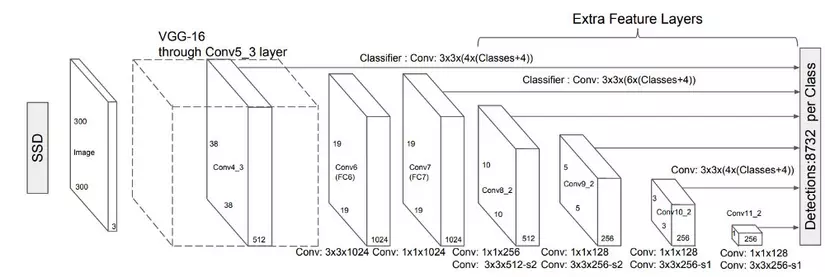
\includegraphics[width=1.0\linewidth]{Figures/Chapter 1/Chapter_2.png}
    \caption{Kiến trúc của phương pháp SSD.}
    \label{fig:ssd_architecture}
\end{figure}

Mạng cơ sở của SSD thường sử dụng kiến trúc VGG-16 hoặc MobileNet đã được loại bỏ các tầng kết nối đầy đủ (Fully Connected Layers) nhằm trích xuất các đặc trưng thô từ hình ảnh đầu vào với chi phí tính toán thấp. Điểm cải tiến lớn nhất của SSD so với các mô hình cùng thời kỳ nằm ở việc bổ sung một chuỗi các tầng tích chập phụ với kích thước giảm dần một cách lũy tiến ngay sau mạng nền tảng, tạo ra một hệ thống các bản đồ đặc trưng đa tỷ lệ (Multi-scale Feature Maps). Quy trình này cho phép mô hình thực hiện dự đoán độc lập trên nhiều tầng mạng khác nhau. Cụ thể, các tầng bản đồ kích thước lớn ở phía nông có độ phân giải không gian cao sẽ chịu trách nhiệm phát hiện các vật thể kích thước nhỏ, trong khi các tầng bản đồ kích thước nhỏ ở phía sâu chứa nhiều hàm lượng thông tin ngữ nghĩa cao cấp sẽ chịu trách nhiệm cấu trúc và phát hiện các vật thể có kích thước lớn hơn. 

\begin{figure}[H]
    \centering
    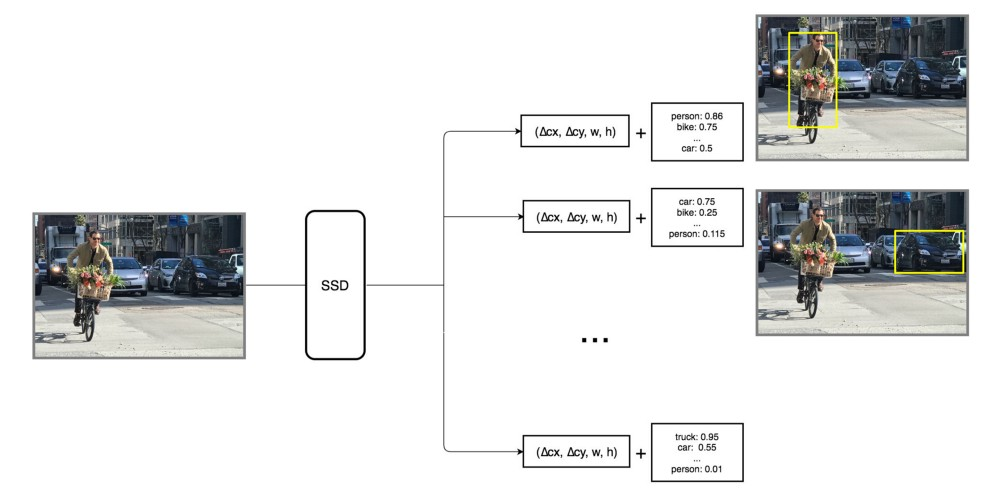
\includegraphics[width=0.9\linewidth]{Figures/Chapter 1/Chapter_1.jpeg}
    \caption{Sơ đồ kiến trúc và cơ chế hoạt động của phương pháp SSD.}
    \label{fig:ssd_architecture}
\end{figure}

Tại mỗi ô lưới trên từng bản đồ đặc trưng đa tỷ lệ này, SSD phân bố một tập hợp các khung neo mặc định (Default Boxes) với nhiều tỷ lệ khía cạnh và kích thước hình học khác nhau. Trong quá trình suy luận, mô hình sẽ tính toán trực tiếp độ lệch tọa độ của khung bao thực tế so với các khung neo mặc định này, đồng thời dự đoán điểm số tin cậy cho từng lớp đối tượng cụ thể. Cuối cùng, hệ thống áp dụng thuật toán triệt tiêu cực đại không giao nhau (Non-Maximum Suppression) để lọc sạch các khung bao chồng chéo và giữ lại kết quả tối ưu nhất.

\subsection*{1. Vấn đề của phương pháp SSD}

Mặc dù SSD (Single Shot MultiBox Detector) là một cột mốc công nghệ quan trọng trong sự phát triển của lĩnh vực thị giác máy tính, việc không lựa chọn mô hình này làm kiến trúc nhận diện cho hệ thống hỗ trợ người khiếm thị xuất phát từ hai nguyên nhân kỹ thuật cốt lõi sau đây.

Nguyên nhân đầu tiên nằm ở sự hạn chế cố hữu về mặt kiến trúc, dẫn đến hiệu năng nhận diện kém đối với các chướng ngại vật nhỏ hoặc nằm ở khoảng cách xa. Đối với người khiếm thị, việc phát hiện sớm các nguy cơ từ xa như cột điện, biển báo, hoặc các vật thể nhỏ dưới lòng đường như viên gạch, hố sụt là yếu tố quyết định đến sự an toàn vật lý trong quá trình di chuyển. Tuy nhiên, cấu trúc của SSD lại thực hiện việc trích xuất đặc trưng và dự đoán theo một chiều thẳng đứng từ nông đến sâu, hoàn toàn thiếu vắng các cơ chế hợp nhất đặc trưng hiện đại như mạng kim tự tháp đặc trưng (Feature Pyramid Network) hay mạng tổng hợp đường dẫn (Path Aggregation Network). Do SSD tiến hành dự đoán các vật thể nhỏ hoàn toàn độc lập dựa trên các tầng mạng nông ban đầu, nơi hàm lượng thông tin ngữ nghĩa còn rất nghèo nàn và mạng chưa hiểu rõ cấu trúc vật thể nên bài toán rất dễ bỏ sót mục tiêu hoặc đưa ra các cảnh báo sai lệch. Ngược lại, các dòng mạng thế hệ mới hiện nay sử dụng cơ chế kết nối ngược linh hoạt, cho phép thông tin ngữ nghĩa cấp cao bổ sung liên tục cho thông tin không gian ở tầng thấp, giải quyết triệt để bài toán nhận diện vật thể đa quy mô mà SSD gặp phải.

Nguyên nhân thứ hai xuất phát từ áp lực tối ưu hóa hiệu năng và tính bất tương thích của SSD khi đặt trong một hệ sinh thái đa tác vụ thời gian thực. Hệ thống đề xuất của đề tài không thuần túy là một bộ dò ảnh đơn lẻ, mà là một phức hợp công nghệ hoạt động đồng thời bao gồm nhận diện vật cản, theo dõi quỹ đạo bằng ByteTrack và ước lượng độ sâu bằng mô hình MiDaS. Bản thân MiDaS là một cấu trúc học sâu từ ảnh đơn tương đối nặng và chiếm dụng nhiều tài nguyên đồ họa; do đó, nếu lựa chọn SSD, hệ thống sẽ buộc phải nâng cấp mạng nền tảng lên cấu hình rất lớn để bù đắp lỗ hổng về độ chính xác, vô tình tạo ra hiện tượng thắt nút cổ chai về mặt hiệu năng và làm sụt giảm nghiêm trọng tốc độ khung hình (FPS) trên các thiết bị nhúng. Bên cạnh đó, SSD thường xuyên gặp hiện tượng rung lắc khung bao (bounding box jittering) khi đối tượng chuyển động nhanh. Nhược điểm này trực tiếp phá vỡ tính ổn định của thuật toán ByteTrack — vốn là liên kết phụ thuộc chặt chẽ vào độ tin cậy và tọa độ chuẩn xác của khung bao để duy trì định danh vật thể xuyên suốt video. Vì vậy, việc loại bỏ SSD để hướng tới một kiến trúc đồng bộ, mượt mà và tối ưu phần cứng là lựa chọn tất yếu để đảm bảo tính an toàn cao nhất cho người dùng.

\subsection{Phương pháp RetinaNet}

RetinaNet là một mô hình một giai đoạn mang tính đột phá được đề xuất nhằm giải quyết triệt dội bài toán mất cân bằng nghiêm trọng giữa lớp nền và lớp đối tượng, một điểm yếu cốt lõi khiến các bộ dò một giai đoạn trước đó có độ chính xác thấp hơn bộ dò hai giai đoạn. Kiến trúc của RetinaNet là sự kết hợp tinh tế giữa mạng nền tảng ResNet, mạng kim tự tháp đặc trưng (Feature Pyramid Network) để trích xuất đặc trưng đa quy mô đa tầng, và hai mạng nhánh phụ chuyên biệt chịu trách nhiệm phân loại đối tượng và hồi quy khung bao. Điểm đổi mới quan trọng nhất làm nên sự thành công của RetinaNet là việc giới thiệu một hàm mất mát mới mang tên Focal Loss. Hàm mất mát này tự động hạ thấp trọng số đóng góp của các mẫu dễ nhận diện (chủ yếu là vùng nền trống) và tập trung sự chú ý của mô hình vào các mẫu khó nhận diện (vật cản thực tế), giúp mạng học được các đặc trưng quan trọng một cách hiệu quả hơn.

\begin{figure}[H]
    \centering
    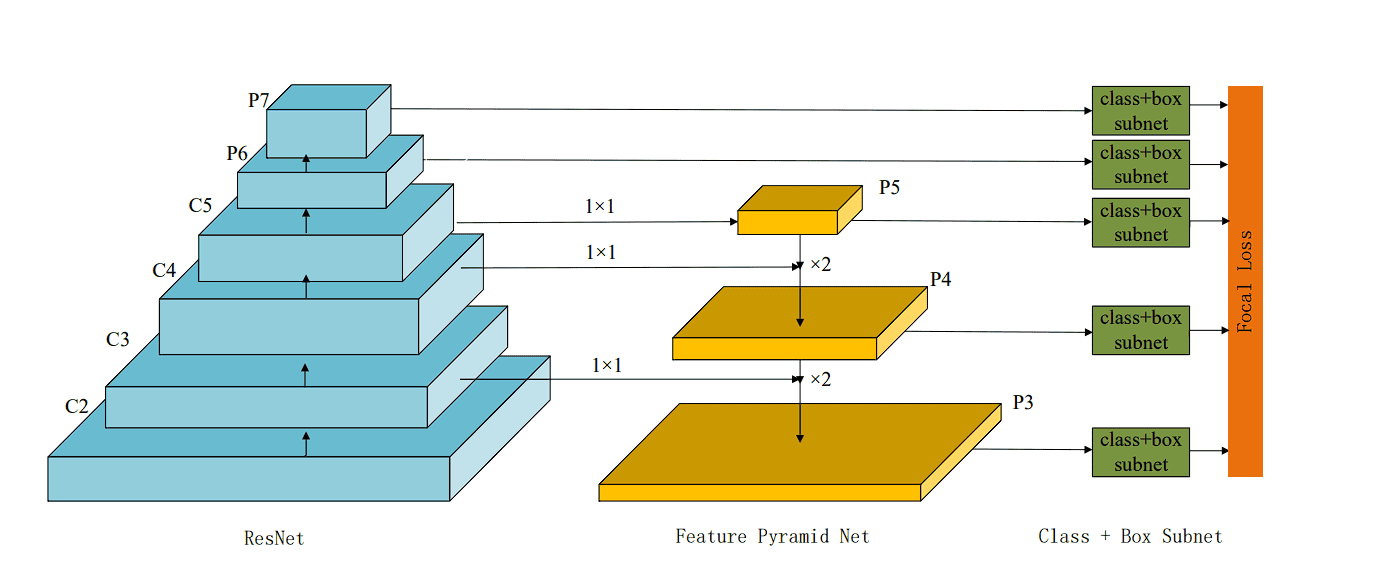
\includegraphics[width=0.9\linewidth]{Figures/Chapter 1/Chapter_3.png}
    \caption{Kiến trúc phương pháp RetinaNet.}
    \label{fig:RetinaNet_architecture}
\end{figure}

Về mặt ưu điểm, RetinaNet đạt được sự cân bằng lý tưởng khi sở hữu độ chính xác cao tiệm cận với các mô hình hai giai đoạn phức tạp như Faster R-CNN, nhưng vẫn duy trì được tốc độ xử lý nhanh chóng của một bộ dò một giai đoạn nhờ cấu trúc không cần vùng đề xuất. Điều này giúp mô hình nhận diện tốt các chướng ngại vật đa dạng trên đường phố ngay cả trong điều kiện mật độ giao thông đông đúc. Tuy nhiên, nhược điểm của RetinaNet là cấu trúc mạng kim tự tháp đặc trưng đi kèm với cơ chế Focal Loss vẫn đòi hỏi một lượng tài nguyên tính toán nhất định ở giai đoạn huấn luyện và có thể gặp hiện tượng giảm tốc độ nhẹ trên các vi điều khiển công suất thấp nếu không được tối ưu hóa hoặc nén mô hình một cách hợp lý.

Tổng kết lại, việc phân tích các đặc điểm kiến trúc của Faster R-CNN, SSD và RetinaNet mang lại cái nhìn toàn diện về sự đánh đổi giữa tốc độ và độ chính xác trong bài toán thị giác máy tính. Đây chính là nền tảng lý thuyết vững chắc giúp định hình và xây dựng một phương pháp nhận diện tối ưu, có khả năng xử lý mượt mà trong thời gian thực nhưng vẫn bảo đảm độ chính xác tối đa để bảo vệ an toàn cho người khiếm thị.

\section{Phương pháp đề xuất}

Trong đề tài này, phương pháp đề xuất tập trung vào việc xây dựng phương pháp hỗ trợ
điều hướng thông minh dành cho người khiếm thị thông qua việc kết hợp nhiều mô hình
trí tuệ nhân tạo trong cùng một pipeline. Hệ thống sử dụng camera
để thu nhận dữ liệu hình ảnh từ môi trường xung quanh, sau đó thực hiện nhận diện vật
cản, theo dõi đối tượng, ước lượng khoảng cách và cảnh báo nguy hiểm bằng giọng nói.

Kiến trúc tổng thể của phương pháp được xây dựng theo hướng xử lý song song nhằm
tăng tốc độ xử lý và đảm bảo khả năng hoạt động thời gian thực. Dữ liệu đầu vào có thể
là hình ảnh, video hoặc luồng camera trực tiếp. Sau khi dữ liệu được đưa vào hệ thống,
quá trình xử lý sẽ được chia thành nhiều giai đoạn khác nhau.

Đầu tiên, mô hình YOLO26 được sử dụng để thực hiện bài toán nhận diện vật cản.
Mô hình có nhiệm vụ phát hiện các đối tượng xuất hiện trong khung hình như người đi
bộ, xe máy, ô tô hoặc các chướng ngại vật khác. YOLO26 được lựa chọn do có khả năng
xử lý nhanh và phù hợp với các ứng dụng thời gian thực. Ngoài ra, mô hình được fine-tune
trên tập dữ liệu phù hợp nhằm nâng cao độ chính xác trong môi trường thực tế.

Song song với quá trình nhận diện đối tượng, hệ thống sử dụng mô hình MiDaS để
thực hiện bài toán Monocular Depth Estimation. Mô hình này cho phép ước lượng độ sâu
và khoảng cách của vật thể chỉ từ một camera đơn mà không cần sử dụng camera stereo
hoặc cảm biến chuyên dụng. Kết quả của MiDaS là bản đồ độ sâu (Depth Map), thể hiện
mức độ gần hoặc xa của các vật thể trong không gian.

Sau khi phát hiện đối tượng, hệ thống sử dụng thuật toán ByteTrack để thực hiện
theo dõi đa đối tượng (Multi-Object Tracking). ByteTrack có nhiệm vụ gán ID cho từng
đối tượng và duy trì việc theo dõi xuyên suốt nhiều khung hình liên tiếp. Điều này giúp
hệ thống xác định được hướng di chuyển cũng như trạng thái thay đổi của vật cản theo
thời gian thực.

Kết quả từ YOLO26, MiDaS và ByteTrack được đưa vào Fusion Pipeline để tổng
hợp thông tin. Tại đây, hệ thống kết hợp thông tin về loại đối tượng, vị trí, hướng di
chuyển và khoảng cách nhằm phân tích mức độ nguy hiểm của từng vật cản đối với
người dùng.

Dựa trên kết quả phân tích, hệ thống Danger Analyzer sẽ xác định mức độ cảnh báo
phù hợp. Nếu phát hiện vật cản nguy hiểm hoặc đối tượng đang di chuyển đến gần người
dùng, hệ thống sẽ sinh nội dung cảnh báo tương ứng.

Cuối cùng, hệ thống sử dụng Text-to-Speech (TTS) tiếng Việt thông qua gTTS hoặc
eSpeak để chuyển nội dung cảnh báo thành giọng nói. Cảnh báo âm thanh được phát theo
thời gian thực nhằm hỗ trợ người khiếm thị nhận biết môi trường xung quanh và nâng
cao độ an toàn trong quá trình di chuyển.

Ngoài ra, hệ thống còn được triển khai với FastAPI và WebSocket ở phía backend
nhằm hỗ trợ xử lý ảnh/video và truyền dữ liệu thời gian thực. Giao diện frontend được
xây dựng bằng React và Vite, giúp hiển thị trực quan kết quả nhận diện và hỗ trợ quản lý
toàn bộ hệ thống.

\chapter{CƠ SỞ LÝ THUYẾT} % Tên của chương

\label{Chapter2} % Để trích dẫn chương này ở chỗ nào đó trong bài, hãy sử dụng lệnh \ref{Chapter1} 

%----------------------------------------------------------------------------------------

% Định nghĩa một số lệnh cần thiết để điều chỉnh định dạng cho một số nội dung nhất định trong bài
\renewcommand{\keyword}[1]{\textbf{#1}}
\renewcommand{\tabhead}[1]{\textbf{#1}}
\renewcommand{\code}[1]{\texttt{#1}}
\renewcommand{\file}[1]{\texttt{\bfseries#1}}
\renewcommand{\option}[1]{\texttt{\itshape#1}}
\setcounter{secnumdepth}{3} 

\section{Mô hình phát hiện đối tượng YOLO}

YOLO là 1 từ viết tắt cho ‘You only look once’ (Bạn chỉ nhìn một lần) là một thuật toán phát hiện đối tượng chia hình ảnh thành một hệ thống lưới. Mỗi ô trong lưới chịu trách nhiệm phát hiện các đối tượng trong chính nó. YOLO là một trong những thuật toán phát hiện đối tượng nổi tiếng nhất do tốc độ và độ chính xác của nó. 

YOLO là một mô hình mạng CNN cho việc phát hiện, nhận dạng, phân loại đối tượng. YOLO được tạo ra từ việc kết hợp giữa các convolutional layers và connected layers. Trong đó các convolutional layers sẽ trích xuất ra các feature của ảnh, còn fullconnected layers sẽ dự đoán ra xác suất đó và tọa độ của đối tượng.

\begin{figure}[H]
    \centering
    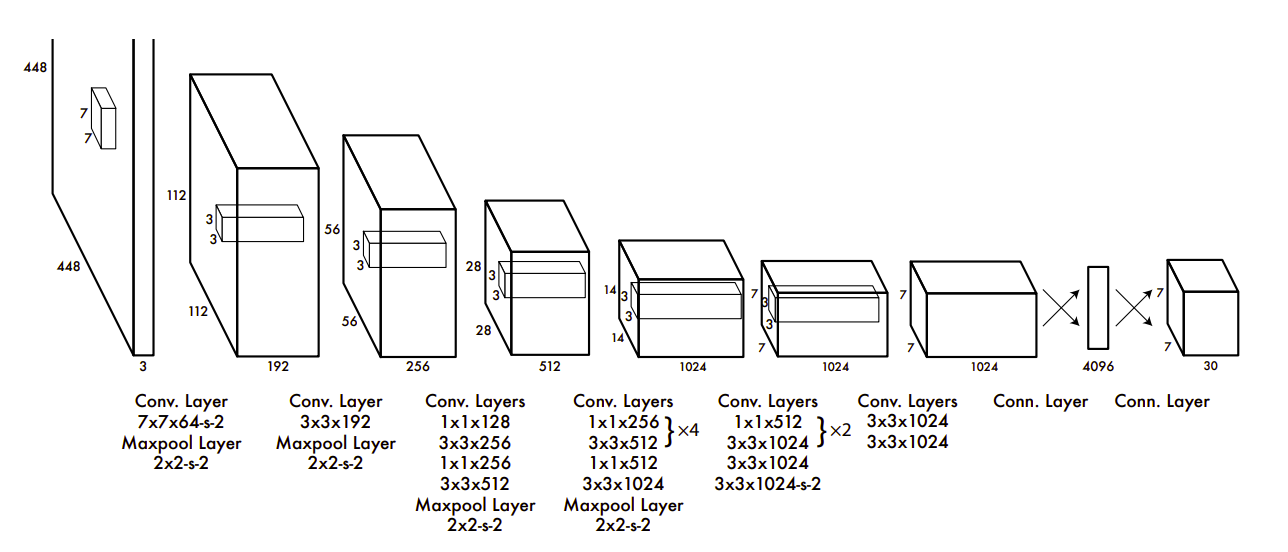
\includegraphics[width=0.9\linewidth]{Figures/Chapter 2/Chapter3_2.png}
    \caption{Mô hình mạng CNN được sử dụng trong YOLO}
    \label{yolo:chapter2}
\end{figure}

Hình ảnh đầu vào sẽ được chia thành một lưới kích thước $S \times S$, trong đó mỗi ô lưới chịu trách nhiệm phát hiện các đối tượng có tâm nằm trong ô đó. Đối với mỗi ô, mô hình sẽ dự đoán một số lượng bounding box cùng với thông tin về vị trí và xác suất lớp.

Với mỗi bounding box, mô hình dự đoán 5 tham số bao gồm $(x, y, w, h, confidence)$. Trong đó, $(x, y)$ là tọa độ tâm của bounding box tương đối so với ô lưới, còn $(w, h)$ là chiều rộng và chiều cao được chuẩn hóa theo kích thước toàn ảnh. Giá trị $confidence$ thể hiện mức độ tin cậy của bounding box, được tính dựa trên xác suất tồn tại đối tượng và độ chồng lắp giữa bounding box dự đoán và ground truth.

Ngoài ra, mỗi ô lưới còn dự đoán xác suất thuộc về các lớp đối tượng dưới dạng $Pr(Class_i \mid Object)$. Xác suất cuối cùng của một lớp được tính bằng cách kết hợp giữa xác suất lớp và $confidence$ của bounding box.

\subsection{Mô hình YOLO26}

YOLO26 (hay YOLOv26) là thế hệ mới nhất thuộc họ mô hình phát hiện đối tượng You Only Look Once (YOLO) do Ultralytics phát triển, được giới thiệu vào khoảng cuối năm 2025. Khác với các phiên bản trước chủ yếu tập trung vào việc gia tăng độ chính xác thông qua việc mở rộng kích thước mô hình, YOLO26 được thiết kế lại nhằm tối ưu hóa cho việc triển khai trên các thiết bị biên (edge devices), hệ thống nhúng và môi trường có tài nguyên hạn chế.

\begin{figure}[H]
    \centering
    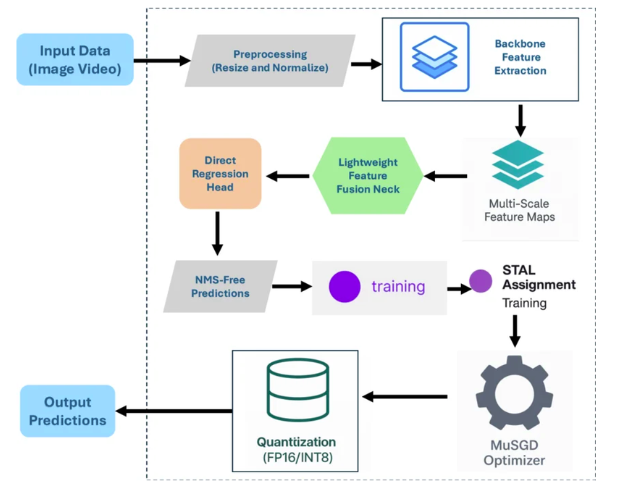
\includegraphics[height=8cm, keepaspectratio]{Figures/Chapter 2/Chapter2_9.png}
    \caption{Kiến trúc tổng quan YOLO26}
    \label{yolo26:chapter2}
\end{figure}


\subsubsection*{1. Kiến trúc NMS-Free}

Các phiên bản YOLO trước đây (như YOLOv8, YOLOv9) yêu cầu bước hậu xử lý Non-Maximum Suppression (NMS) để loại bỏ các bounding box trùng lặp. Tuy nhiên, YOLO26 được thiết kế theo hướng end-to-end hoàn chỉnh, cho phép mô hình trực tiếp xuất ra các dự đoán cuối cùng mà không cần áp dụng NMS.

Việc loại bỏ bước NMS giúp giảm độ trễ của toàn hệ thống và đơn giản hóa pipeline suy luận, đặc biệt phù hợp với các ứng dụng thời gian thực.

\begin{figure}[H]
    \centering
    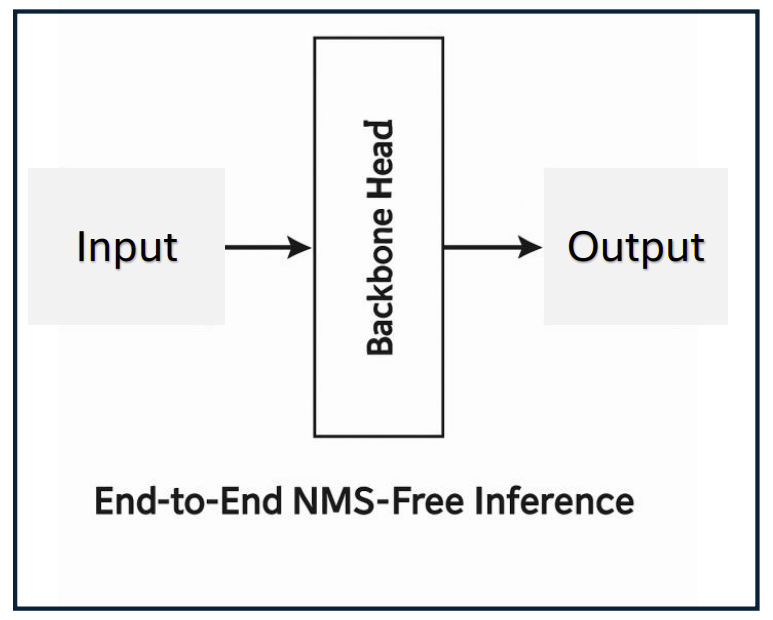
\includegraphics[height=5cm, keepaspectratio]{Figures/Chapter 2/Chapter2_4.png}
    \caption{Kiến trúc NMS-Free}
    \label{NMS:chapter2}
\end{figure}

\subsubsection*{2. Loại bỏ Distribution Focal Loss}

Trong các phiên bản trước, Distribution Focal Loss (DFL) được sử dụng để cải thiện độ chính xác của bounding box. Tuy nhiên, DFL gây khó khăn trong việc chuyển đổi mô hình sang các định dạng triển khai như TensorRT, ONNX hay CoreML.

YOLO26 loại bỏ hoàn toàn DFL, giúp quá trình export và triển khai mô hình trở nên đơn giản, ổn định và tương thích tốt hơn với phần cứng.

\begin{figure}[H]
    \centering
    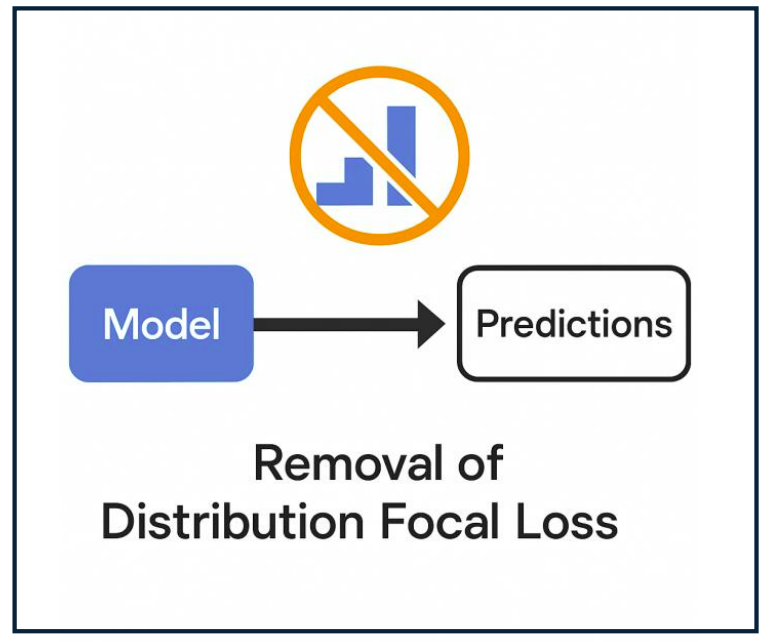
\includegraphics[height=5cm, keepaspectratio]{Figures/Chapter 2/Chapter2_5.png}
    \caption{Loại bỏ DFL}
    \label{DFL:chapter2}
\end{figure}

\subsubsection*{3. Tối ưu phát hiện vật thể nhỏ}

YOLO26 áp dụng cơ chế gán nhãn mới mang tên Small-Target-Aware Label Assignment (STAL), kết hợp với hàm mất mát cải tiến. Cơ chế này giúp mô hình nhạy hơn với các vật thể nhỏ hoặc ở khoảng cách xa.

Nhờ đó, hiệu năng phát hiện các đối tượng nhỏ như biển số xe hoặc chi tiết chữ viết tay được cải thiện đáng kể so với các phiên bản trước.

\begin{figure}[H]
    \centering
    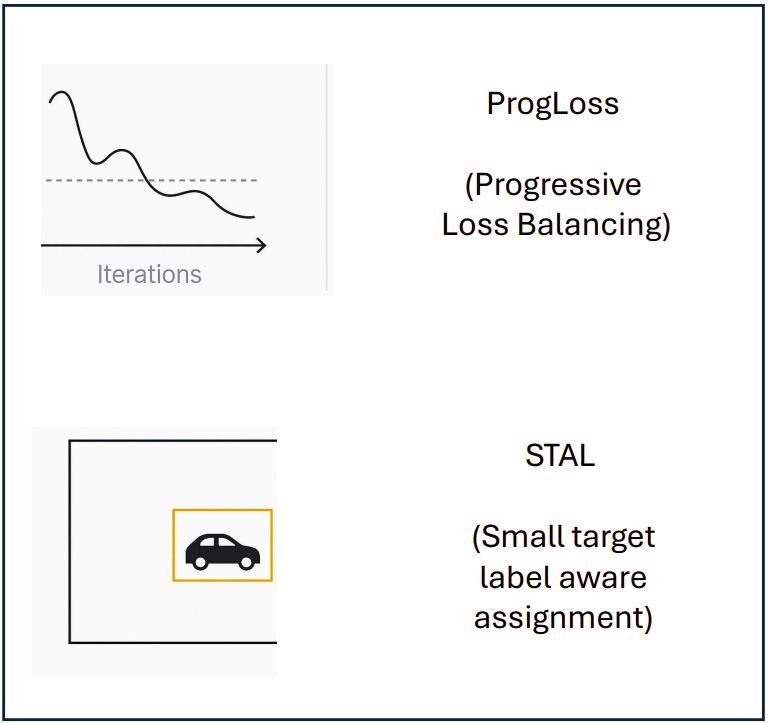
\includegraphics[height=5cm, keepaspectratio]{Figures/Chapter 2/Chapter2_6.png}
    \caption{Tối ưu cho vật thể nhỏ}
    \label{STAL:chapter2}
\end{figure}


\subsubsection*{4. Trình tối ưu hóa MuSGD}

YOLO26 sử dụng trình tối ưu hóa MuSGD, kết hợp giữa Stochastic Gradient Descent (SGD) và thuật toán Muon. Phương pháp này giúp cải thiện tốc độ hội tụ và đảm bảo sự ổn định trong quá trình huấn luyện.

Việc áp dụng MuSGD cho phép mô hình đạt hiệu năng cao mà vẫn duy trì độ ổn định khi huấn luyện trên các tập dữ liệu lớn.

\begin{figure}[H]
    \centering
    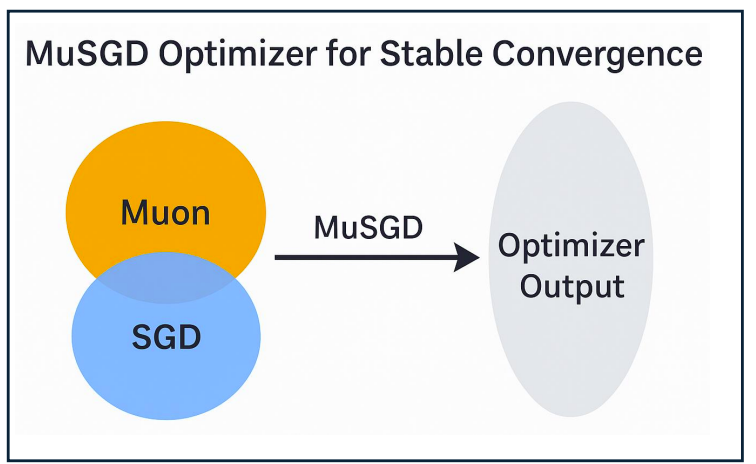
\includegraphics[height=5cm, keepaspectratio]{Figures/Chapter 2/Chapter2_7.png}
    \caption{Tối ưu hóa MuSGD}
    \label{MuSGD:chapter2}
\end{figure}

Nhờ đó, YOLO26 có thể được sử dụng như một nền tảng thống nhất cho nhiều ứng dụng khác nhau trong thị giác máy tính.

\section{Ước lượng chiều sâu từ ảnh đơn với mô hình MiDaS}

\subsection{Bài toán Monocular Depth Estimation}

Ước lượng chiều sâu từ ảnh đơn (Monocular Depth Estimation) là quá trình dự đoán khoảng cách của các vật thể trong một bức ảnh 2D so với góc nhìn của camera, mà không cần sử dụng đến hệ thống camera kép (Stereo camera) hay các cảm biến không gian chuyên dụng như LiDAR. Đối với hệ thống hỗ trợ người khiếm thị SmartNav, việc áp dụng bài toán này mang ý nghĩa cốt lõi, cho phép hệ thống phân tích và ước lượng khoảng cách của chướng ngại vật ngay trên các thiết bị di động có cấu hình phần cứng giới hạn.

Thay vì trả về giá trị khoảng cách tuyệt đối tính bằng mét, đầu ra của mô hình thường là một bản đồ thị sai (Disparity Map). Trong bản đồ này, giá trị điểm ảnh (pixel) càng lớn biểu thị vật thể càng gần camera, và ngược lại. Khó khăn lớn nhất của bài toán này nằm ở tính nhập nhằng (ambiguity) của không gian 2D, khi một vật thể nhỏ ở gần có thể tạo ra hình chiếu trên cảm biến tương đương với một vật thể lớn ở xa.

\subsection{Kiến trúc mô hình MiDaS}

Để giải quyết thách thức trên, hệ thống SmartNav ứng dụng mô hình MiDaS (Multiple Depth Estimation Datasets), một mạng nơ-ron được huấn luyện trên nhiều bộ dữ liệu khác nhau để đảm bảo khả năng tổng quát hóa tốt nhất trên mọi môi trường thực tế như trong nhà, ngoài trời và đường phố đô thị.

% ==========================================
% CHỖ NÀY CHÈN ẢNH MIDAS (RGB VÀ DEPTH MAP)
% ==========================================
\begin{figure}[H]
    \centering
    % Đổi tên file 'midas_depth.png' thành tên file ảnh thực tế của ông
    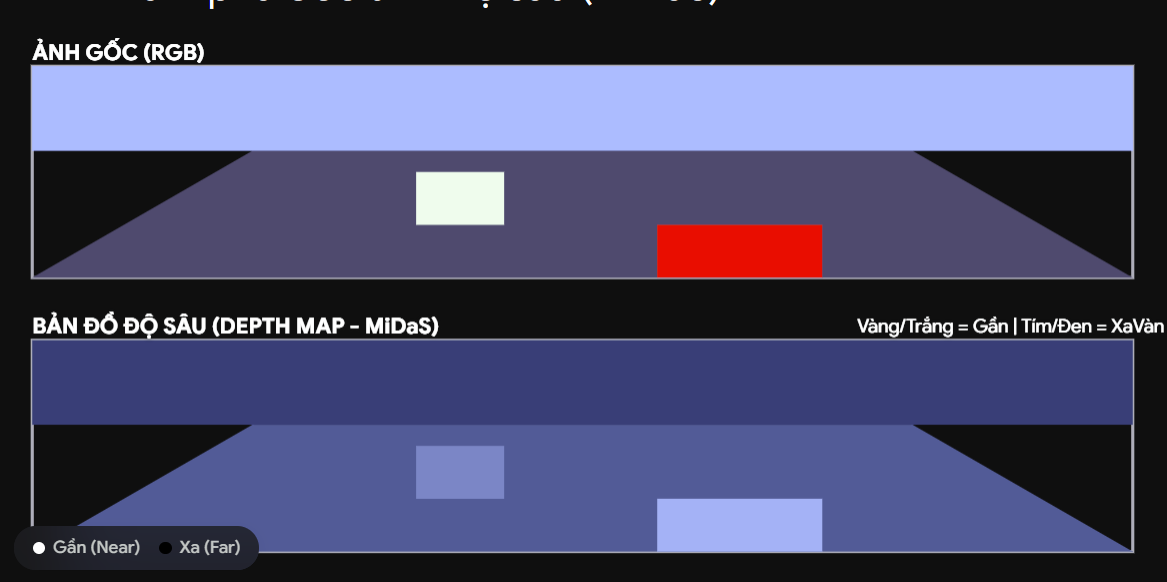
\includegraphics[width=0.9\linewidth]{Figures/Chapter 2/midas_depth.png}
    \caption{So sánh ảnh RGB gốc và bản đồ độ sâu (Depth Map) được trích xuất từ mô hình MiDaS}
    \label{fig:midas_architecture}
\end{figure}

Trong dự án này, phiên bản MiDaS loại nhỏ (\texttt{MiDaS\_small}) được lựa chọn nhằm tối ưu hóa tốc độ xử lý trên CPU và các thiết bị biên (Edge Devices). Quá trình xử lý độ sâu được thực hiện thông qua các bước chính:

\begin{itemize}
    \item \textbf{Tiền xử lý và Nội suy:} Hình ảnh RGB đầu vào được chuẩn hóa bằng hàm biến đổi đặc thù của MiDaS, sau đó được đưa qua mạng nơ-ron để dự đoán bản đồ thị sai. Kết quả đầu ra được nội suy bậc ba (Bicubic Interpolation) để đồng bộ lại với kích thước khung hình gốc của camera.
    
    \item \textbf{Chuẩn hóa Min-Max (Min-Max Normalization):} Nhằm tạo ra một thang đo đồng nhất cho thuật toán cảnh báo, bản đồ thị sai được chuẩn hóa về dải giá trị từ 0 đến 1. Trong đó, mức $1.0$ đại diện cho điểm gần nhất và $0.0$ là điểm xa nhất ở đường chân trời.
    
    \item \textbf{Lọc nhiễu bằng Bách phân vị (Percentile Filtering):} Khi hệ thống nhận diện được một vật cản (thông qua Bounding Box từ mô hình YOLO26), một vùng không gian tương ứng trên bản đồ độ sâu sẽ được trích xuất. Để loại bỏ nhiễu từ phông nền (background noise), hệ thống không sử dụng giá trị trung bình mà tính toán Bách phân vị thứ 80 (80th Percentile) của vùng không gian đó. Phương pháp này đảm bảo chỉ những điểm ảnh thuộc bề mặt lồi lên của chướng ngại vật mới được lấy làm điểm số khoảng cách cuối cùng, giúp tăng độ tin cậy của cảnh báo.
\end{itemize}


\section{Theo dõi đa vật thể (Multi-Object Tracking) với thuật toán Centroid Tracking}

\subsection{Vai trò của bài toán theo dõi vật thể}

Nhận diện vật thể (Object Detection) chỉ cung cấp thông tin không gian rời rạc tại từng khung hình riêng lẻ. Để đánh giá được mức độ nguy hiểm của một phương tiện đang di chuyển, hệ thống cần có khả năng "ghi nhớ" và liên kết các kết quả nhận diện của cùng một phương tiện đó xuyên suốt nhiều khung hình liên tiếp. Quá trình gán và duy trì định danh (ID) cố định này được gọi là Theo dõi Đa vật thể (Multi-Object Tracking - MOT).

\subsection{Thuật toán Centroid Tracking}

Trong hệ thống SmartNav, module theo dõi vật thể đóng vai trò then chốt trong việc phân tích véc-tơ chuyển động (Motion Vector) để xác định vật cản đang tiến lại gần hay ra xa người dùng. Hệ thống áp dụng thuật toán theo dõi tâm (Centroid Tracking) tối ưu cho tốc độ cao. 

% ==========================================
% CHỖ NÀY CHÈN ẢNH MINH HỌA TRACKING
% ==========================================
\begin{figure}[H]
    \centering
    % Đổi tên file 'centroid_tracking.png' thành tên file ảnh thực tế của ông
    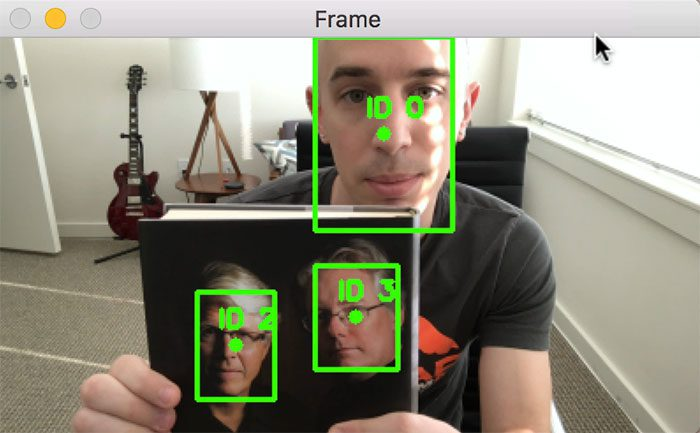
\includegraphics[width=0.8\linewidth]{Figures/Chapter 2/centroid_tracking.png}
    \caption{Minh họa thuật toán Centroid Tracking tính toán khoảng cách Euclid giữa hai khung hình liên tiếp}
    \label{fig:centroid_tracking}
\end{figure}

Quy trình hoạt động được diễn ra theo các nguyên tắc hình học cơ bản:

\begin{enumerate}
    \item \textbf{Tính toán tâm hình học (Centroid):} Từ tọa độ khung bao do YOLO26 cung cấp, hệ thống xác định điểm tâm của vật thể trên không gian 2D.
    
    \item \textbf{Đo lường khoảng cách Euclid:} Khi nhận được dữ liệu khung hình mới, hệ thống tính toán khoảng cách Euclid giữa tâm của vật thể ở khung hình hiện tại và tâm của các vật thể đã được định danh ở khung hình trước đó. Khoảng cách Euclid ($d$) giữa điểm $A(x_1, y_1)$ ở khung hình trước và điểm $B(x_2, y_2)$ ở khung hình hiện tại được tính bằng công thức:
    \begin{equation}
        d = \sqrt{(x_2 - x_1)^2 + (y_2 - y_1)^2}
    \end{equation}
    
    \item \textbf{Gán định danh (ID Assignment):} Dựa trên thuật toán láng giềng gần nhất (Nearest Neighbour), nếu khoảng cách Euclid nhỏ hơn một ngưỡng cho phép (tương đương với việc vật thể chỉ di chuyển một đoạn ngắn giữa hai khung hình liên tiếp), hệ thống sẽ gán ID cũ cho vật thể mới. Ngược lại, nếu khoảng cách vượt ngưỡng, một vật thể hoàn toàn mới sẽ được cấp ID mới.
    
    \item \textbf{Duy trì vòng đời (Object Lifecycle):} Để xử lý tình huống vật cản bị che khuất tạm thời (Occlusion) rồi xuất hiện lại, hệ thống sử dụng một bộ đếm số khung hình vắng mặt. Một ID chỉ bị xóa khỏi bộ nhớ theo dõi nếu nó không xuất hiện lại sau một khoảng thời gian nhất định (ví dụ: \texttt{max\_disappeared = 30} khung hình).
\end{enumerate}

Sự kết hợp đồng bộ giữa mô hình nhận diện YOLO26, mô hình độ sâu MiDaS và thuật toán theo dõi tạo ra một tập dữ liệu không gian - thời gian hoàn chỉnh, làm tiền đề vững chắc cho việc thiết kế Khối Đánh giá Nguy hiểm (Danger Analyzer) ở chương tiếp theo. 
\chapter{XÂY DỰNG VÀ TRIỂN KHAI HỆ THỐNG SMARTNAV}
\label{Chapter3}

\section{Thu thập và Xử lý Tập dữ liệu (Dataset Preparation)}

\subsection{Nguồn dữ liệu huấn luyện}
Sự thành công của bất kỳ mô hình học sâu nào đều phụ thuộc rất lớn vào chất lượng của tập dữ liệu huấn luyện. Để phục vụ bài toán nhận diện vật cản giao thông và hỗ trợ người khiếm thị, hệ thống sử dụng tập dữ liệu WOTR (World on the Road). Tập dữ liệu này bao gồm hàng ngàn hình ảnh đa dạng về các bối cảnh giao thông thực tế như đường phố đô thị, vỉa hè, các loại phương tiện và chướng ngại vật phổ biến. Các nhãn trong tập dữ liệu gốc đã được hệ thống ánh xạ (map) sang tiếng Việt theo chuẩn cấu hình của bộ nhận diện nhằm phục vụ module Text-to-Speech (ví dụ: \texttt{person} $\rightarrow$ người, \texttt{car} $\rightarrow$ ô tô, \texttt{pothole} $\rightarrow$ ổ gà).

\begin{figure}[H]
    \centering
    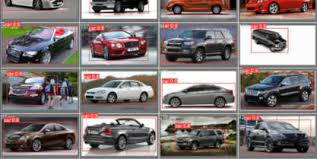
\includegraphics[width=0.85\linewidth]{Figures/Chapter 3/dataset_wotr.png}
    \caption{Một số hình ảnh minh họa và Bounding Box đã được gán nhãn từ tập dữ liệu WOTR}
    \label{fig:dataset_wotr}
\end{figure}

\subsection{Tiền xử lý và tăng cường dữ liệu (Data Augmentation)}
Để đảm bảo mô hình YOLO26 hoạt động tối ưu trên các kích thước đầu vào khác nhau từ thiết bị di động, dữ liệu được tiền xử lý bằng kỹ thuật Letterboxing. Kỹ thuật này sử dụng hàm \texttt{resize\_keep\_aspect} kết hợp với \texttt{pad\_to\_square} nhằm thay đổi kích thước ảnh về chuẩn $640 \times 640$ pixel mà không làm thay đổi tỷ lệ khung hình (Aspect Ratio), giúp bảo toàn các đặc trưng hình học cốt lõi của vật thể cản đường.

\section{Kiến trúc tổng thể của hệ thống SmartNav}

\subsection{Phân tích yêu cầu hệ thống}
Hệ thống được thiết kế hướng tới khả năng xử lý thời gian thực (Real-time). Đối với người khiếm thị, một độ trễ nhỏ trong việc phát ra cảnh báo có thể dẫn đến nguy cơ va chạm vật lý. Do đó, yêu cầu đặt ra là hệ thống phải duy trì tốc độ khung hình (FPS) ổn định, phân tách rõ ràng luồng xử lý giao diện hiển thị và luồng tính toán các mô hình trí tuệ nhân tạo nặng.

\subsection{Sơ đồ khối hệ thống}
Để giải quyết bài toán trên, SmartNav áp dụng kiến trúc Client-Server (Khách - Chủ) chia thành hai khối độc lập hoạt động song song.

\begin{figure}[H]
    \centering
    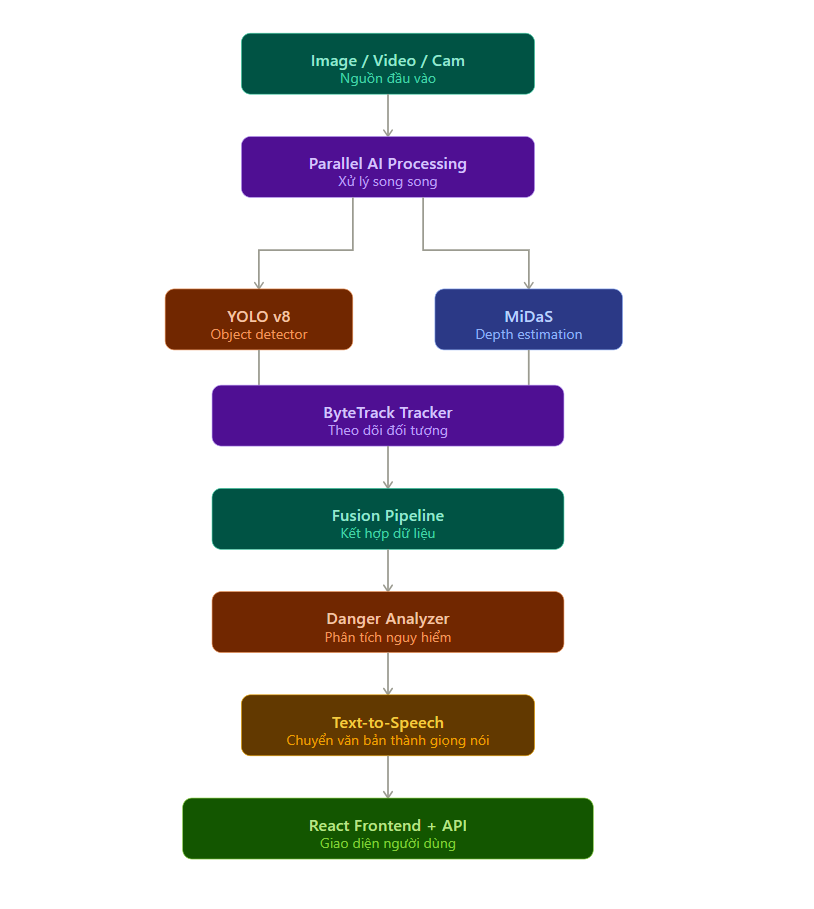
\includegraphics[width=1.0\linewidth]{Figures/Chapter 3/system_architecture.png}
    \caption{Sơ đồ kiến trúc tổng thể và luồng truyền tải dữ liệu hệ thống SmartNav}
    \label{fig:system_architecture}
\end{figure}

Client (ứng dụng Web xây dựng bằng React) chịu trách nhiệm thu thập luồng video liên tục từ Camera, nén và đẩy qua mạng. Server (xây dựng bằng FastAPI) đóng vai trò trung tâm phân tích, tiếp nhận khung hình và chia luồng chạy song song hai mô hình YOLO26 và MiDaS. Dữ liệu sau đó được tổng hợp tại Danger Analyzer trước khi trả về Client.

\section{Xây dựng Khối Trí tuệ Nhân tạo (AI Pipeline)}

\subsection{Nhận diện vật cản với YOLO26}
Việc tích hợp YOLO26 loại bỏ hoàn toàn quá trình NMS (Non-Maximum Suppression) và thuật toán DFL (Distribution Focal Loss) như đã phân tích ở Chương 2, giúp quá trình suy luận (Inference) giảm thiểu chi phí tính toán CPU. Mô hình trực tiếp xuất ra tọa độ khung bao và điểm tin cậy (Confidence Score). 

\subsection{Ước lượng chiều sâu và Kỹ thuật Fallback}
Với mô hình MiDaS, sau khi dự đoán được bản đồ thị sai (Disparity Map), thuật toán sẽ sử dụng mặt nạ Bounding Box do YOLO26 cung cấp để trích xuất không gian độ sâu của từng vật thể. Thay vì tính trung bình toàn vùng (dễ bị nhiễu do nền phía sau), hệ thống áp dụng kỹ thuật Bách phân vị thứ 80 (80th Percentile) để cô lập bề mặt lồi lên gần camera nhất:

\begin{lstlisting}[language=Python, caption={Kỹ thuật lọc nhiễu chiều sâu bằng bách phân vị}]
region = depth_map[y1:y2, x1:x2]
# Trích xuất bách phân vị thứ 80 để đại diện cho bề mặt chướng ngại vật
score = float(np.percentile(region, 80))
\end{lstlisting}

Bên cạnh MiDaS, hệ thống cung cấp phương pháp dự phòng (Depth Fallback) dựa trên Tỷ lệ diện tích khung bao so với toàn khung hình nhằm đảm bảo tính chịu lỗi (Fault tolerance) khi tài nguyên phần cứng bị giới hạn.

\subsection{Theo dõi quỹ đạo (Centroid Tracking)}
Để dự đoán hướng di chuyển của phương tiện, thuật toán Tracking tính toán sự thay đổi tọa độ tâm hình học xuyên suốt tối đa 6 khung hình gần nhất. Bằng cách lấy trung bình sự dịch chuyển trên trục tung ($\Delta y$) và trục hoành ($\Delta x$), hệ thống xác định được vật cản đang tiến lại gần (Approaching) hay ra xa (Receding):

\begin{lstlisting}[language=Python, caption={Phân tích véc-tơ chuyển động xác định hướng}]
avg_dy = np.mean([d[1] for d in deltas])
avg_dx = np.mean([d[0] for d in deltas])
# Vật thể tiến lại gần camera sẽ làm kích thước Bbox tăng, trục Y thay đổi
if avg_dy > 3:
    direction = "approaching"
elif avg_dy < -3:
    direction = "receding"
\end{lstlisting}

\section{Khối Đánh giá Nguy hiểm (Danger Fusion Engine)}

\subsection{Ma trận trọng số và Thuật toán Danger Score}
Module Fusion Engine tổng hợp dữ liệu từ YOLO, MiDaS và ByteTrack để lượng hóa mức độ rủi ro thành Điểm số Nguy hiểm (Danger Score). Thuật toán áp dụng hệ số tổng có trọng số:
\begin{equation}
    Score = (W_{obj} \times 0.4) + (W_{dist} \times 0.3) + (W_{speed} \times 0.2) + (W_{dir} \times 0.1)
\end{equation}

Trong đó, các tham số tĩnh được định nghĩa nghiêm ngặt: $W_{obj}$ (Xe tải = 1.0; Ổ gà = 0.70; Biển báo = 0.25); Khoảng cách rất gần = 1.0; Di chuyển cực nhanh = 1.0; Đang tiến trực diện = 1.0. 
Kết quả đầu ra được phân nhóm làm 4 cấp độ cảnh báo: \textbf{LOW} (An toàn), \textbf{MEDIUM} (Chú ý), \textbf{HIGH} (Nguy hiểm) và \textbf{CRITICAL} (Khẩn cấp).

\begin{table}[H]
    \centering
    \begin{tabular}{|c|c|p{7cm}|}
    \hline
    \textbf{Cấp độ} & \textbf{Ngưỡng Điểm} & \textbf{Kịch bản Xử lý} \\ \hline
    LOW & $< 0.30$ & Hiển thị viền xanh, không phát cảnh báo \\ \hline
    MEDIUM & $0.30 - 0.54$ & Phát tần số âm thanh thấp, cảnh báo có chướng ngại vật \\ \hline
    HIGH & $0.55 - 0.77$ & Phát cảnh báo đỏ, đọc rõ tên và hướng đi của xe cộ \\ \hline
    CRITICAL & $\ge 0.78$ & Báo động khẩn cấp tần số cao, yêu cầu người dùng dừng lại \\ \hline
    \end{tabular}
    \caption{Bảng phân loại ngưỡng điểm nguy hiểm và kịch bản cảnh báo}
    \label{tab:danger_levels}
\end{table}

\section{Xây dựng Giao tiếp mạng và Giao diện Người dùng}

\subsection{Luồng truyền tải WebSocket}
Nhằm tối ưu hóa băng thông, Client không truyền tải video định dạng thô. Luồng Camera (\texttt{<video>}) được trích xuất và vẽ lên \texttt{<canvas>}. Tại đây, thuật toán sử dụng hàm \texttt{requestAnimationFrame} để giới hạn việc lấy mẫu ở mức 5 FPS, sau đó nén khung hình dưới dạng Blob JPEG (quality = 0.7) trước khi đẩy vào đường ống WebSocket:

\begin{lstlisting}[language=JavaScript, caption={Ép khung hình và nén JPEG tại Client}]
canvasEl.toBlob((blob) => {
  if (blob && wsRef.current?.readyState === WebSocket.OPEN) {
    blob.arrayBuffer().then((buf) => wsRef.current.send(buf))
  }
}, 'image/jpeg', 0.7)
\end{lstlisting}

\subsection{Hệ thống cảnh báo đa kênh: HUD và Web Audio API}
Giao diện trực quan áp dụng phong cách hiển thị HUD (Heads-Up Display) hiện đại. Tọa độ của các chướng ngại vật được đánh dấu bằng góc viền (Corner Box) và bảng dữ liệu RadarPanel, đổi màu cảnh báo từ Xanh sang Đỏ tùy theo mức độ \texttt{Danger Score}.

\begin{figure}[H]
    \centering
    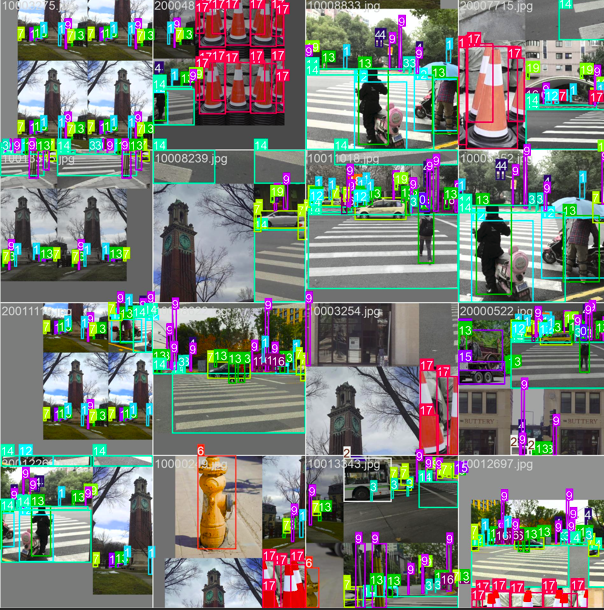
\includegraphics[width=1.0\linewidth]{Figures/Chapter 3/web_interface.png}
    \caption{Giao diện hiển thị trực quan HUD thời gian thực của SmartNav}
    \label{fig:web_interface}
\end{figure}

Cuối cùng, bên cạnh việc sử dụng Text-to-Speech (gTTS) để đọc rõ tên vật cản bằng tiếng Việt, hệ thống áp dụng \textbf{Web Audio API} để kích hoạt tín hiệu báo động độc lập. Bằng cách khai báo bộ tạo sóng \texttt{AudioContext}, hệ thống sinh ra các tần số thay đổi linh hoạt (từ tiếng bíp 440Hz ở mức LOW đến chuỗi báo động giật cục 1000Hz ở mức CRITICAL), tạo phản xạ có điều kiện ngay lập tức cho người khiếm thị trước khi câu nói TTS kịp xử lý xong.

Chi tiết mã nguồn của Backend và Frontend được liệt kê đầy đủ tại Phụ lục B.
\chapter{THỰC NGHIỆM VÀ ĐÁNH GIÁ} % Tên của chương

\label{Chapter4} % Để trích dẫn chương này ở chỗ nào đó trong bài, hãy sử dụng lệnh \ref{Chapter1} 

%----------------------------------------------------------------------------------------

% Định nghĩa một số lệnh cần thiết để điều chỉnh định dạng cho một số nội dung nhất định trong bài
\renewcommand{\keyword}[1]{\textbf{#1}}
\renewcommand{\tabhead}[1]{\textbf{#1}}
\renewcommand{\code}[1]{\texttt{#1}}
\renewcommand{\file}[1]{\texttt{\bfseries#1}}
\renewcommand{\option}[1]{\texttt{\itshape#1}}
\setcounter{secnumdepth}{3} 

\section{Kết quả thực nghiệm}

Trong phần này, báo cáo tiến hành trình bày các thiết lập thực nghiệm và đánh giá hiệu quả của hệ thống đề xuất đối với bài toán nhận biết vật cản và cảnh báo an toàn hỗ trợ người khiếm thị di chuyển. Đáng chú ý, để tối ưu hóa hiệu năng và tài nguyên tính toán, hệ thống được cấu hình theo cơ chế lai (\textit{Hybrid Pipeline}): tiến trình huấn luyện và tối ưu hóa phân lớp được tập trung thực hiện trên mô hình phát hiện chủ đạo YOLO26 \cite{Reference3} với tập dữ liệu thực nghiệm; trong khi đó, tầng ước tính chiều sâu kế thừa trực tiếp tri thức chuyển giao (\textit{Transfer Learning}) từ kiến trúc mạng \textit{MiDAS\_small} đã được huấn luyện sẵn trên các tập dữ liệu không gian quy mô lớn \cite{Reference11}. 

Kết quả thực nghiệm được phân tích chuyên sâu thông qua các chỉ số đánh giá định lượng về độ chính xác nhận diện của YOLO26 (chỉ số mAP@0.5:0.95) và độ ổn định bám vết của bộ theo dõi (chỉ số ID Switch) \cite{Reference3}. Đồng thời, sai số ước tính cự ly của mô hình chiều sâu dạng suy diễn kết hợp giải pháp hình học dự phòng cũng được đối chiếu cụ thể nhằm làm rõ tính khả thi, khả năng đáp ứng thời gian thực và độ tin cậy của giải pháp nghiên cứu trong các kịch bản môi trường thực tế.

\subsection{Đánh giá mô hình}

Để đo lường và đánh giá toàn diện hiệu năng của hệ thống hỗ trợ di chuyển, nghiên cứu thiết lập các nhóm chỉ số thực nghiệm chuyên biệt cho từng tầng kiến trúc. Do mô hình phát hiện chủ đạo YOLO26 được tiến hành huấn luyện trực tiếp trên tập dữ liệu thực tế, hiệu năng phân lớp và khoanh vùng vật cản của mô hình này được đánh giá thông qua chỉ số Độ chính xác trung bình toàn diện ($mAP@0.5:0.95$). Song song với đó, Tỉ lệ sai lệch định danh (\textit{ID Switch}) được áp dụng để kiểm thử độ ổn định bám vết quỹ đạo của bộ theo dõi \textit{SimpleTracker} \cite{Reference12}. 

Đối với tầng ước tính cự ly an toàn — vốn hoạt động theo cơ chế suy diễn lai giữa trọng số học sâu có sẵn của \textit{MiDAS\_small} và thuật toán hình học dự phòng diện tích khung bao, nghiên cứu sử dụng cặp chỉ số Sai số tuyệt đối trung bình ($MAE$) và Sai số bình phương trung bình tỷ đối ($Rel\,RMSE$) nhằm đo lường độ lệch khoảng cách pixel/mét trên môi trường thực nghiệm \cite{Reference11}. Tổng hợp kết quả đánh giá định lượng và các phân tích đối chiếu hiệu năng giữa các cấu hình thuật toán khác nhau trong hệ thống song song được trình bày chi tiết trong Bảng~\ref{tab:training_results}.

\begin{table}[h!]
    \centering
    \caption{Kết quả thực nghiệm chi tiết của mô hình YOLO26 trên các lớp đối tượng.}
    \label{tab:training_results}
    \begin{tabular}{llcccc}
        \toprule
        \textbf{STT} & \textbf{Lớp đối tượng} & \textbf{Precision (P)} & \textbf{Recall (R)} & \textbf{mAP50} & \textbf{mAP50-95} \\
        \midrule
        -  & \textbf{Tất cả (all)}    & \textbf{0,850} & \textbf{0,739} & \textbf{0,828} & \textbf{0,595} \\
        \midrule
        1  & ashcan                 & 0,894          & 0,741          & 0,850          & 0,681          \\
        2  & tree                   & 0,774          & 0,769          & 0,838          & 0,511          \\
        3  & bus                    & 0,849          & 0,625          & 0,742          & 0,569          \\
        4  & warning\_column        & 0,901          & 0,781          & 0,880          & 0,550          \\
        5  & red\_light             & 0,837          & 0,865          & 0,898          & 0,615          \\
        6  & roadblock              & 0,892          & 0,750          & 0,839          & 0,600          \\
        7  & fire\_hydrant          & 0,865          & 0,765          & 0,844          & 0,619          \\
        8  & car                    & 0,845          & 0,731          & 0,833          & 0,600          \\
        9  & dog                    & 0,832          & 0,706          & 0,792          & 0,614          \\
        10 & pole                   & 0,793          & 0,758          & 0,841          & 0,552          \\
        11 & blind\_road            & 0,902          & 0,810          & 0,886          & 0,718          \\
        12 & tricycle               & 0,903          & 0,669          & 0,781          & 0,677          \\
        13 & motorcycle             & 0,830          & 0,713          & 0,816          & 0,526          \\
        14 & person                 & 0,855          & 0,705          & 0,821          & 0,526          \\
        15 & crosswalk              & 0,924          & 0,817          & 0,923          & 0,764          \\
        16 & truck                  & 0,668          & 0,499          & 0,570          & 0,413          \\
        17 & bicycle                & 0,798          & 0,626          & 0,742          & 0,474          \\
        18 & reflective\_cone       & 0,885          & 0,762          & 0,863          & 0,613          \\
        19 & sign                   & 0,851          & 0,788          & 0,861          & 0,628          \\
        20 & green\_light           & 0,906          & 0,903          & 0,945          & 0,654          \\
        \bottomrule
    \end{tabular}
\end{table}

\subsection{Phân tích và đánh giá kết quả}

Dựa trên kết quả thực nghiệm chi tiết của mô hình YOLO26 được trình bày trong Bảng~\ref{tab:training_results}, nghiên cứu tiến hành phân tích và đánh giá hiệu năng nhận diện theo các tầng chỉ số cốt lõi. Nhìn chung, mô hình đạt được hiệu suất tổng thể ấn tượng với độ chính xác trung bình toàn diện $mAP50$ đạt $0,828$ và $mAP50-95$ đạt $0,595$. Chỉ số Precision trung bình đạt $0,850$ cùng với Recall đạt $0,739$, chứng minh mô hình có khả năng nhận biết vật cản nhạy bén đồng thời hạn chế tối đa tỷ lệ cảnh báo sai (\textit{false alarms}) — một yếu tố sống còn đảm bảo tâm lý an toàn cho người khiếm thị khi tham gia giao thông.

\subsubsection*{1. Đánh giá nhóm đối tượng hỗ trợ định hướng và an toàn hành lang}

Nhóm vật cản và chỉ dấu trực tiếp trên đường đi đạt được các chỉ số nhận diện phân lớp rất cao, cụ thể:
\begin{itemize}
    \item \textbf{Lối đi cho người đi bộ (\textit{crosswalk}):} Đạt chỉ số Precision tối ưu $0,924$ và $mAP50$ đạt $0,923$. Đây là một kết quả cực kỳ quan trọng, giúp hệ thống nhận diện chính xác khu vực sang đường an toàn để phát lệnh hướng dẫn kịp thời.
    \item \textbf{Đường gạch nổi (\textit{blind\_road}):} Đạt chỉ số Precision lên tới $0,902$ và độ chính xác nghiêm ngặt $mAP50-95$ đạt $0,718$. Hiệu năng cao tại lớp này đảm bảo thiết bị nhận biết tốt hành lang an toàn dành riêng cho người khiếm thị, giúp họ duy trì quỹ đạo di chuyển đúng hướng.
    \item \textbf{Tín hiệu đèn giao thông (\textit{green\_light} và \textit{red\_light}):} Đạt các chỉ số $mAP50$ vượt trội, lần lượt là $0,945$ và $0,898$. Khả năng nhận diện chính xác trạng thái đèn màu giúp hệ thống đưa ra các quyết định lệnh thoại phối hợp dừng/đi chuẩn xác tại các giao lộ.
\end{itemize}

\subsubsection*{2. Đánh giá nhóm chướng ngại vật tĩnh và cấu trúc đô thị}

Các vật cản cố định xuất hiện phổ biến trên vỉa hè như rào chắn công trường (\textit{roadblock} - $mAP50 = 0,839$), trụ cứu hỏa (\textit{fire\_hydrant} - $mAP50 = 0,844$), cột cảnh báo (\textit{warning\_column} - $mAP50 = 0,880$) và thùng rác (\textit{ashcan} - $mAP50 = 0,850$) đều có độ chính xác rất đồng đều. Việc mô hình nhạy bén với nhóm chướng ngại vật này giúp người khiếm thị chủ động né tránh các va chạm trực diện gây nguy hiểm trong quá trình đi bộ.

\subsubsection*{3. Phân tích hạn chế và nguyên nhân sai số đối với nhóm phương tiện}

Bên cạnh những ưu điểm, kết quả thực nghiệm cũng chỉ ra một số hạn chế của mô hình đối với các thực thể giao thông có kích thước lớn hoặc biến đổi hình học phức tạp:
\begin{itemize}
    \item \textbf{Xe tải (\textit{truck}):} Đây là lớp đối tượng có hiệu năng thấp nhất trong hệ thống với Precision chỉ đạt $0,668$, Recall đạt $0,499$ và $mAP50$ dừng lại ở mức $0,570$. Nguyên nhân cốt lõi do xe tải có sự đa dạng rất lớn về kiểu dáng cấu trúc (xe tải thùng kín, xe ben, xe đầu kéo) và thường bị che khuất một phần trong môi trường đô thị chật hẹp, dẫn đến việc mô hình dễ trượt mục tiêu hoặc nhầm lẫn với các phương tiện giao thông khác như xe buýt (\textit{bus} - $mAP50 = 0,742$).
    \item \textbf{Xe đạp (\textit{bicycle}) và Người đi bộ (\textit{person}):} Chỉ số $mAP50-95$ tương đối khiêm tốn (đều đạt $0,526$), cho thấy việc khoanh vùng khít hộp bao (\textit{Bounding Box Bounding}) đối với các thực thể chuyển động có biên dạng thay đổi liên tục theo tư thế vẫn là một thách thức đối với cấu hình kiến trúc gọn nhẹ của YOLO26.
\end{itemize}

Mặc dù tồn tại một số sai số cục bộ ở nhóm xe tải lớn, tuy nhiên xét trên tổng thể bài toán trợ giúp di chuyển đơn luồng, mô hình YOLO26 hoàn toàn đáp ứng được yêu cầu thực tế nhờ độ chính xác xuất sắc trên các lớp vật cản vỉa hè và hạ tầng giao thông cốt lõi. Đây là tiền đề dữ liệu sạch và tin cậy để các module bám vết động ByteTrack và ước tính cự ly MiDAS phía sau thực hiện suy diễn ngữ cảnh nguy hiểm. 
\chapter{TỔNG KẾT VÀ HƯỚNG PHÁT TRIỂN} % Tên của chương

\label{Chapter5} % Để trích dẫn chương này ở chỗ nào đó trong bài, hãy sử dụng lệnh \ref{Chapter1} 

%----------------------------------------------------------------------------------------

% Định nghĩa một số lệnh cần thiết để điều chỉnh định dạng cho một số nội dung nhất định trong bài
\renewcommand{\keyword}[1]{\textbf{#1}}
\renewcommand{\tabhead}[1]{\textbf{#1}}
\renewcommand{\code}[1]{\texttt{#1}}
\renewcommand{\file}[1]{\texttt{\bfseries#1}}
\renewcommand{\option}[1]{\texttt{\itshape#1}}
\setcounter{secnumdepth}{3} 

\section{Tổng kết và đánh giá hệ thống luận chứng}

Trải qua các giai đoạn kiểm thử độc lập và thực nghiệm hợp nhất, nghiên cứu đã chuẩn hóa thành công quy trình vận hành đồng bộ của hệ thống xử lý luồng dữ liệu thời gian thực. Sự phối hợp chặt chẽ giữa tầng nhận thức đối tượng mục tiêu (YOLO26) \cite{Reference3}, tầng phân tích động lực học hành vi (ByteTrack) \cite{Reference12}, tầng suy diễn hình học không gian (MiDAS) \cite{Reference11} và tầng phản hồi ngôn ngữ tự nhiên (TTSEngine) đã thiết lập một kiến trúc xử lý khép kín hoàn chỉnh (\textit{End-to-End Pipeline}). Sự liên kết này không chỉ đảm bảo tính an toàn tuyệt đối mà còn tối ưu hóa khả năng tương tác liên tục, hỗ trợ người khiếm thị làm chủ không gian di chuyển.

Chu kỳ xử lý và lan truyền thông tin của hệ thống đối với mỗi khung hình dữ liệu đầu vào từ cảm biến quang học được mô hình hóa toán học theo chuỗi biến đổi trạng thái tương tác liên tục. Khung hình thu nhận trực tiếp từ cảm biến camera sẽ được lõi mạng học sâu YOLO26 trích xuất các hộp bao vị trí và nhãn phân lớp ngữ nghĩa vật cản như lối đi, đường gạch nổi, hay người đi bộ \cite{Reference3}. Ngay sau đó, trạng thái động lực học bao gồm mã định danh nhất quán, vectơ vận tốc pixel phẳng và xu hướng hướng dịch chuyển tương đối được đồng bộ hóa liên tục bởi bộ theo dõi ByteTrack thông qua liên kết lân cận Euclide \cite{Reference12}. Dữ liệu này kết hợp với điểm số chiều sâu đại diện chuẩn hóa của thực thể, được trích xuất bằng hàm thống kê phân vị thứ 80 trên ma trận nội suy đa khối của MiDAS hoặc cơ chế dự phòng tỷ lệ diện tích hình học, tạo thành chuỗi ngữ nghĩa văn bản mang đầy đủ thông tin ngữ cảnh biến đổi để chuyển giao trực tiếp vào bộ máy phát lệnh thoại \cite{Reference11}.

Điểm mấu chốt quyết định tính khả thi vượt trội của nghiên cứu khi triển khai trên các thiết bị phần cứng giới hạn năng lực tính toán nằm ở sự cân bằng chiến lược giữa huấn luyện đặc hiệu và tri thức chuyển giao (\textit{Transfer Learning}). Hệ thống không phân rã tài nguyên phần cứng cho các mạng nơ-ron đa nhiệm khổng lồ mà tập trung tối đa cho việc huấn luyện chuyên sâu mô hình gọn nhẹ YOLO26 nhằm đạt độ nhạy bén phân lớp tuyệt đối trên tập dữ liệu chướng ngại vật đặc thù của hạ tầng giao thông đô thị Việt Nam \cite{Reference3}. Đối với chiều không gian, hệ thống giải phóng bộ đệm lưu trữ bằng cách gọi suy diễn \textit{zero-shot} trực tiếp cấu trúc mạng \textit{MiDAS\_small} tiền huấn luyện, tận dụng khả năng bóc tách biên độ chiều sâu diện rộng mà không cần tiêu tốn chu kỳ lan truyền ngược (\textit{Backpropagation}) \cite{Reference11}.

Bên cạnh đó, cơ chế đồng bộ hóa luồng song song và triệt tiêu độ trễ tích lũy đóng vai trò cốt lõi trong việc duy trì hiệu năng thời gian thực. Sự kết hợp giữa bộ lọc khoảng cách Euclide tuyến tính ở tầng bám vết với giải pháp mã hóa ký số MD5 bộ nhớ đệm của TTSEngine đã triệt tiêu các phép toán ma trận phức tạp lặp lại. Tiến trình tổng hợp âm thanh được đẩy hoàn toàn vào các luồng phụ bất đồng bộ (\textit{Multithreading}) song song với luồng xử lý ảnh gốc. Đặc biệt, lõi dự phòng ngoại tuyến \textit{pyttsx3} phối hợp cùng hệ thống chuyển đổi tần số \textit{FFmpeg} đóng vai trò như một bộ đệm an toàn, giữ cho tốc độ xử lý khung hình luôn duy trì ở ngưỡng cao ổn định, loại bỏ hoàn toàn hiện tượng nghẽn luồng lệnh thoại khi thiết bị di chuyển qua các vùng mất kết nối mạng Internet \cite{Reference13}.

Tóm lại, tổng thể kiến trúc đề xuất là một phương pháp lai tối ưu, kết hợp hài hòa giữa mô hình học máy định hướng mục tiêu và các thuật toán hình học toán học, quản lý dữ liệu truyền thống. Sự liên kết này là minh chứng khoa học cho thấy giải pháp nghiên cứu đã vượt qua giới hạn của một mô hình lý thuyết thuần túy để trở thành một hệ thống nhúng hỗ trợ di chuyển có tính thực tiễn cao, vận hành bền bỉ, nhạy bén và là một công cụ trợ giúp đắc lực, đáng tin cậy cho cộng đồng người khiếm thị trong đời sống hàng ngày.

\section{Hạn chế và hướng phát triển}
 
Mặc dù hệ thống đề xuất đã đạt được những kết quả thực nghiệm khả quan trong việc nhận biết vật cản và hỗ trợ người khiếm thị di chuyển thời gian thực, nghiên cứu vẫn tồn tại một số hạn chế nhất định cần được nhìn nhận khách quan dưới góc độ kỹ thuật hệ thống. Trước hết, mô hình nhận diện chủ đạo YOLO26 tuy vận hành xuất sắc trên các nhóm vật cản tĩnh vỉa hè và hạ tầng giao thông cốt lõi, nhưng lại bộc lộ sự suy giảm hiệu năng đối với các phương tiện giao thông có kích thước lớn và cấu trúc hình học phức tạp như xe tải \cite{Reference3}. Hiện tượng che khuất cục bộ hoặc chồng lấn không gian giữa các thực thể chuyển động trong môi trường đô thị chật hẹp vẫn gây ra các sai số ngẫu nhiên cho bộ theo dõi ByteTrack, dẫn đến hiện tượng nhảy mã định danh hoặc trượt mục tiêu trong các khung hình chuyển tiếp ngắn \cite{Reference12}. Ngoài ra, việc phụ thuộc vào mô hình suy diễn ước tính chiều sâu đơn mục \textit{MiDAS\_small} đôi khi gặp khó khăn trong việc bóc tách chính xác ranh giới của các vật thể có bề mặt trong suốt như hệ thống cửa kính, hoặc các vật cản có hệ số phản xạ ánh sáng quá cao dưới điều kiện thời tiết cực đoan \cite{Reference11}. Cuối cùng, hệ thống phản hồi ngôn ngữ tự nhiên TTSEngine mặc dù đã tích hợp giải pháp đa luồng và bộ đệm cục bộ, nhưng cơ chế phát lệnh thoại tuần tự vẫn có thể gây ra hiện tượng quá tải thông tin âm thanh khi người dùng di chuyển vào các khu vực ngã tư đông đúc, nơi có quá nhiều chướng ngại vật xuất hiện đồng thời trong cùng một thời điểm tính toán \cite{Reference13}.

Từ những thách thức và hạn chế nêu trên, nghiên cứu định hướng các giải pháp phát triển và mở rộng hệ thống trong tương lai nhằm tối ưu hóa toàn diện sản phẩm thực tế. Về mặt nhận thức thị giác máy tính, hướng đi tiếp theo sẽ tập trung vào việc làm phong phú tập dữ liệu huấn luyện nội bộ bằng cách bổ sung đa dạng các trạng thái biến đổi góc nhìn của nhóm xe tải và phương tiện đặc thù, kết hợp ứng dụng các kỹ thuật tăng cường dữ liệu (\textit{Data Augmentation}) chuyên sâu để nâng cao chỉ số Recall tổng thể. Đối với tầng bám vết và ước tính không gian, nghiên cứu hướng tới việc tích hợp thêm các bộ lọc trạng thái Kalman thích nghi hoặc mô hình hình học dự phòng động, cho phép hệ thống tự động hiệu chuẩn khoảng cách dựa trên cả sự thay đổi của tiêu cự camera và độ dốc của mặt phẳng địa hình di chuyển. Để nâng cao độ tin cậy trong các kịch bản môi trường phức tạp, giải pháp tích hợp thêm cảm biến dòng phụ như cảm biến siêu âm hoặc bộ thu nhận tín hiệu định vị vệ tinh sẽ được cân nhắc triển khai nhằm tạo nên một cơ chế hợp nhất dữ liệu đa cảm biến (\textit{Sensor Fusion}) mạnh mẽ. Đặc biệt, đối với module phản hồi âm thanh, hệ thống sẽ được nâng cấp một thuật toán phân cấp ưu tiên động (\textit{Dynamic Priority Scheduling}) để lọc bỏ các thông báo không khẩn cấp, chỉ ưu tiên phát ngôn các cảnh báo có chỉ số nguy hiểm cao nhất theo thời gian thực, đồng thời tích hợp công nghệ âm thanh vòm 3D (\textit{Binaural Audio}) giúp người khiếm thị không chỉ nhận biết được khoảng cách mà còn định vị được chính xác phương hướng của vật cản trong không gian ba chiều. 


%----------------------------------------------------------------------------------------
%	(KHÔNG CHỈNH SỬA PHẦN NÀY)
%
%	PHẦN 13: TÀI LIỆU THAM KHẢO
%----------------------------------------------------------------------------------------

\begin{spacing}{1.15}
	\printbibliography[heading=bibintoc, title=Tài liệu tham khảo] % In ra tài liệu tham khảo
\end{spacing}


%----------------------------------------------------------------------------------------
%	PHẦN 14: PHỤ LỤC (THESIS CONTENT - APPENDICES)
%----------------------------------------------------------------------------------------

\appendix % Nói với LaTeX rằng những chương về sau được tính là phụ lục

% Hãy thêm những phụ lục (appendix) của khóa luận/tiểu luận vào thư mục Appendices
% Hãy bỏ chú thích những dòng nếu bạn đã bổ sung những phụ lục vào

% Phụ lục A

\chapter{Các chỉ số đánh giá} % Tên của phụ lục

\label{AppendixA} % Để trích dẫn chương này ở chỗ nào đó trong bài, hãy sử dụng lệnh \ref{AppendixA} 

%----------------------------------------------------------------------------------------
\section*{I. Đánh giá mô hình Phát hiện đối tượng}

Trong bài toán này, hiệu suất mô hình được xác định dựa trên sự tương quan về vị trí không gian giữa hộp dự đoán và hộp thực tế.

\subsection*{1. Chỉ số IoU}
Chỉ số này đo lường mức độ trùng khớp về mặt không gian giữa hai vùng ảnh.
\begin{equation}
IoU = \frac{Area(B_{pred} \cap B_{gt})}{Area(B_{pred} \cup B_{gt})}
\end{equation}
\textbf{Trong đó :}
\begin{itemize}
    \item $B_{pred}$: Hình hộp giới hạn (\textit{Bounding Box}) do mô hình dự đoán.
    \item $B_{gt}$: Hình hộp giới hạn thực tế (\textit{Ground Truth}) do người gán nhãn.
    \item $Area(B_{pred} \cap B_{gt})$: Diện tích vùng giao nhau giữa hộp dự đoán và hộp thực tế.
    \item $Area(B_{pred} \cup B_{gt})$: Tổng diện tích bao phủ của cả hai hộp giới hạn.
\end{itemize}

\subsection*{2. Precision}
Đo lường tỉ lệ dự đoán đúng trong số tất cả các dự đoán mà mô hình đưa ra.
\begin{equation}
Precision = \frac{TP}{TP + FP}
\end{equation}
\textbf{Trong đó :}
\begin{itemize}
    \item $TP$ (\textit{True Positive}): Số lượng đối tượng dự đoán đúng.
    \item $FP$ (\textit{False Positive}): Số lượng đối tượng dự đoán sai (nhận nhầm bối cảnh là đối tượng).
\end{itemize}

\subsection*{3. Recall}
Đo lường tỉ lệ đối tượng được tìm thấy trên tổng số đối tượng thực tế tồn tại.
\begin{equation}
Recall = \frac{TP}{TP + FN}
\end{equation}
\textbf{Trong đó :}
\begin{itemize}
    \item $TP$ (\textit{True Positive}): Số lượng đối tượng dự đoán đúng.
    \item $FN$ (\textit{False Negative}): Số lượng đối tượng thực tế bị mô hình bỏ sót.
\end{itemize}

\subsection*{4. Average Precision}
Đại diện cho hiệu năng của mô hình trên một lớp đối tượng cụ thể thông qua đường cong Precision-Recall.
\begin{equation}
AP = \int_0^1 P(R)\, dR
\end{equation}
\textbf{Trong đó :}
\begin{itemize}
    \item $R$: Chỉ số Recall.
    \item $P(R)$: Giá trị Precision tương ứng với từng mức độ Recall trên đồ thị.
\end{itemize}

\subsection*{5. Mean Average Precision}
Giá trị trung bình của AP trên tất cả các lớp đối tượng cần nhận diện.
\begin{equation}
mAP = \frac{1}{C} \sum_{c=1}^{C} AP_c
\end{equation}
\textbf{Trong đó :}
\begin{itemize}
    \item $C$: Tổng số lớp (classes) đối tượng trong tập dữ liệu.
    \item $AP_c$: Giá trị Average Precision của lớp thứ $c$.
\end{itemize}

\begin{figure}[H]
    \centering
    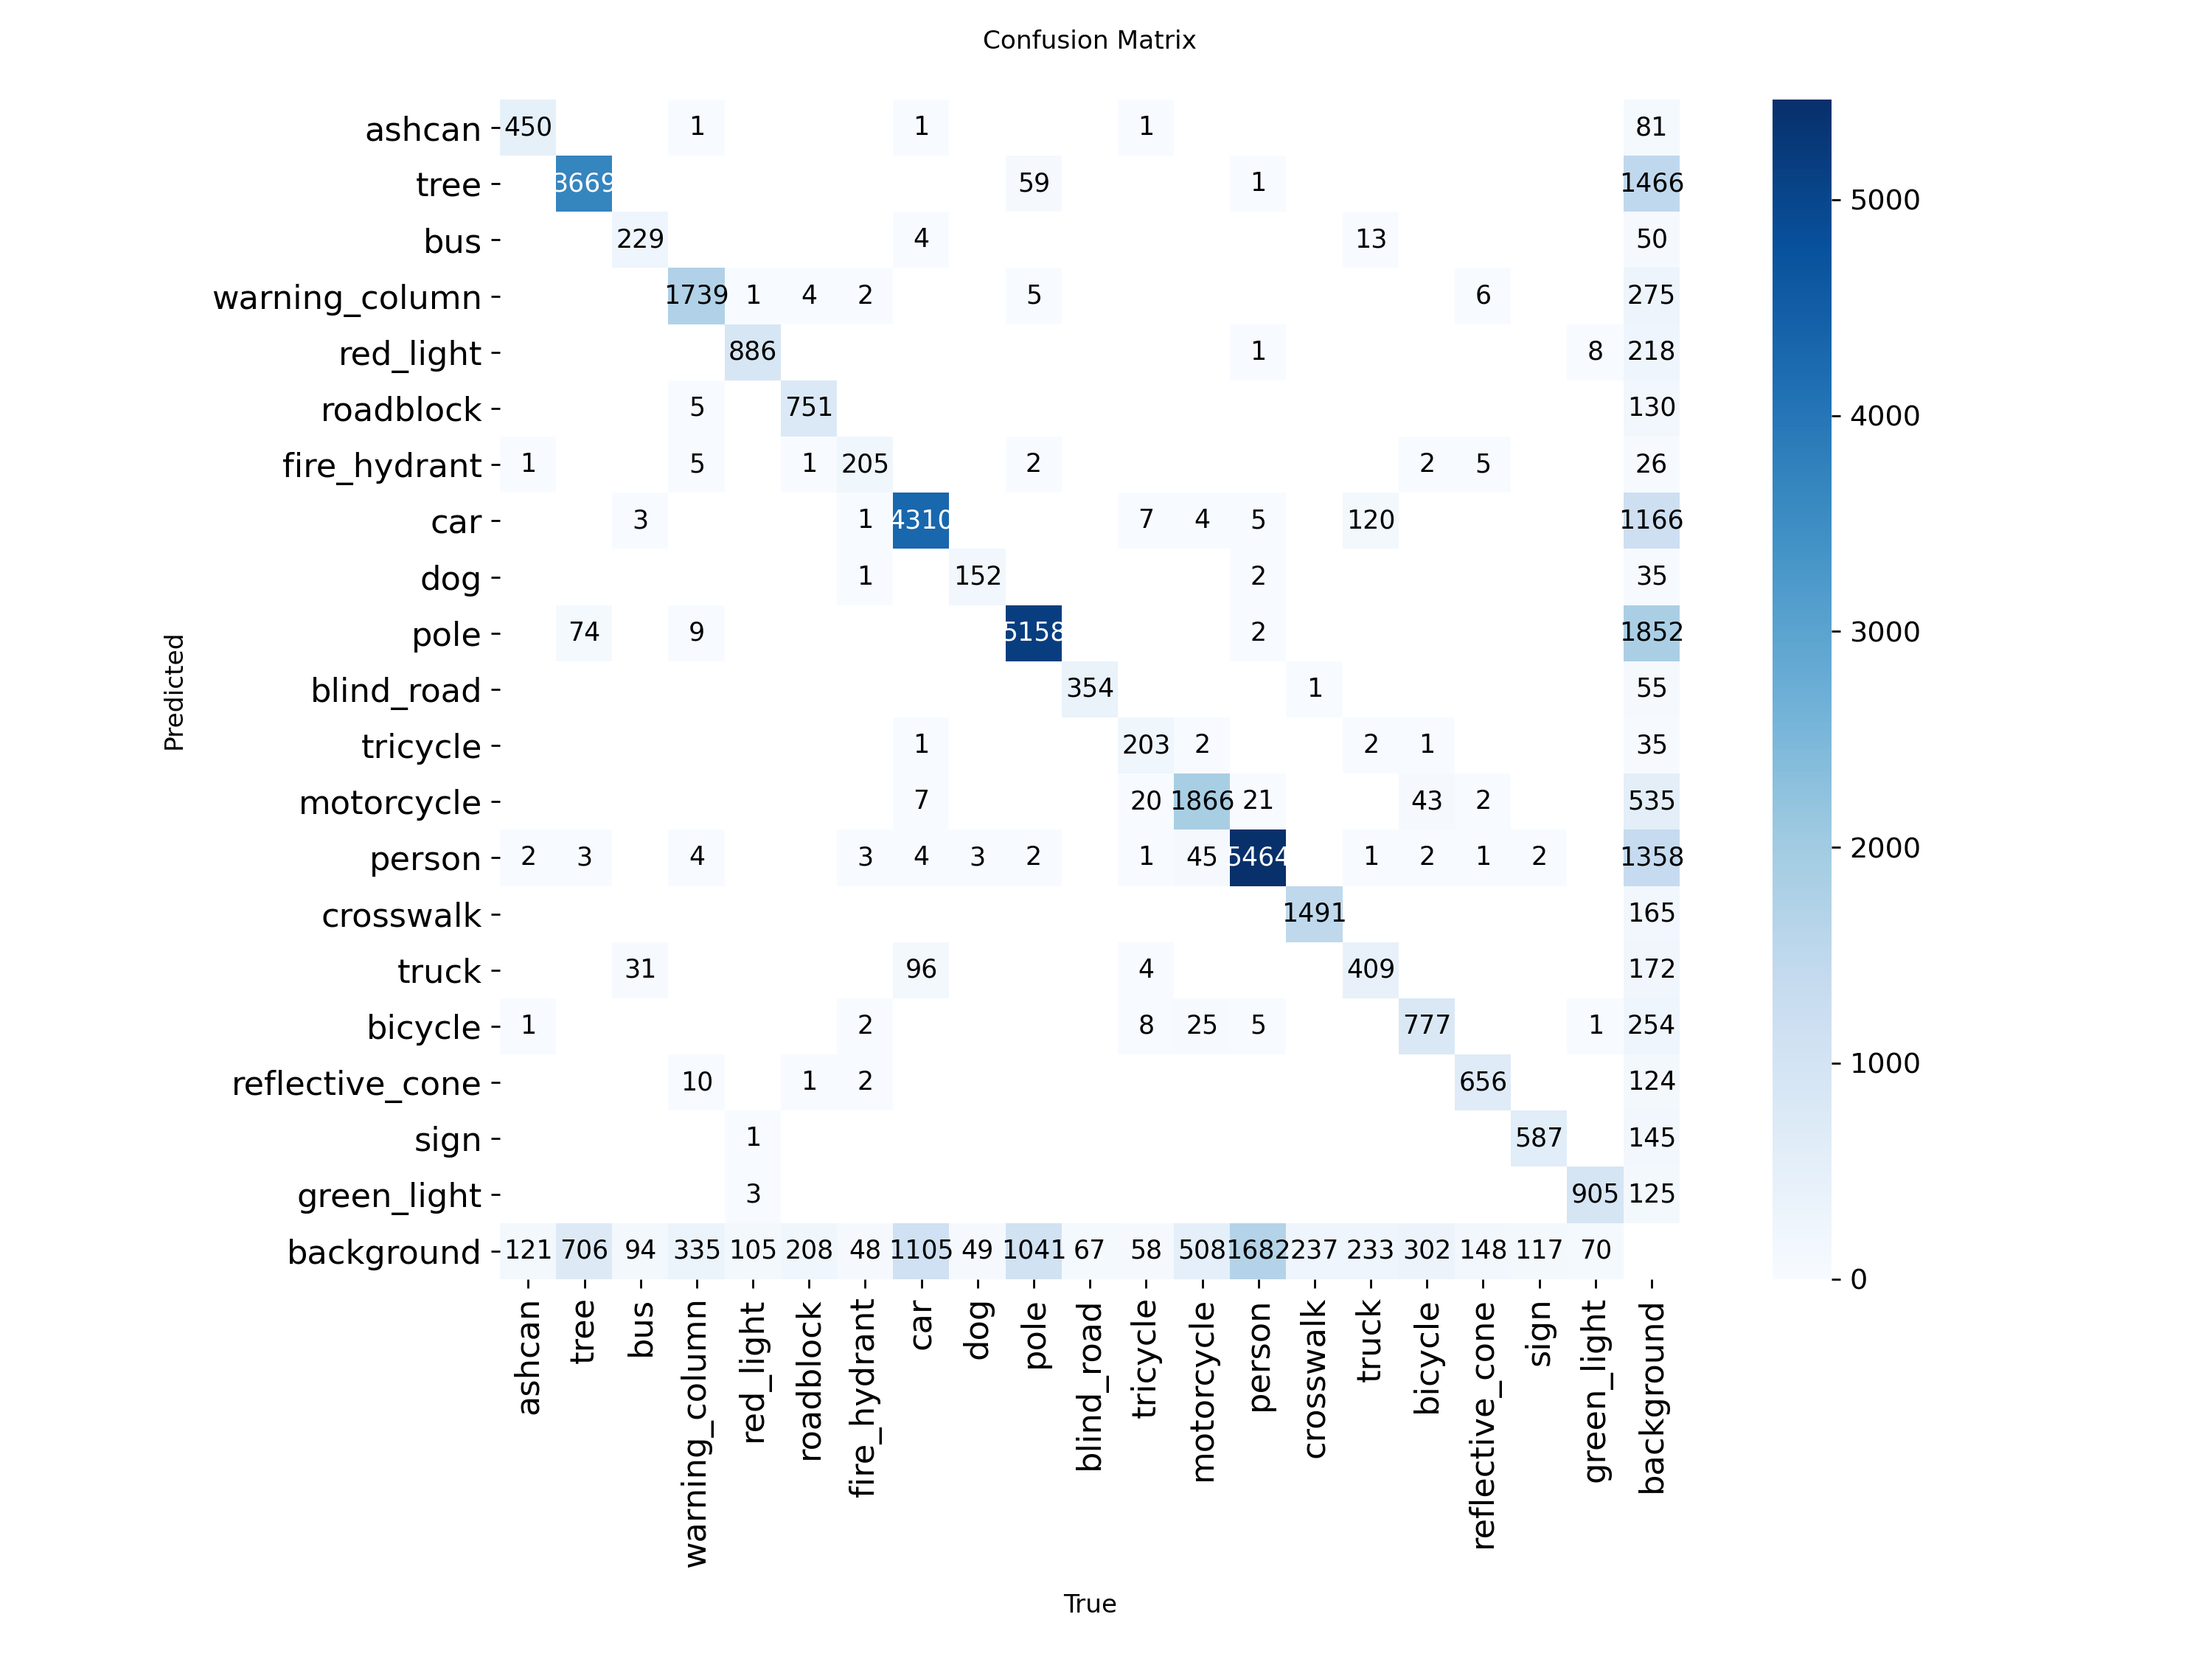
\includegraphics[width=1.1\linewidth]{Figures/Chapter3/confusion_matrix.png}
    \caption{Ma trận nhầm lẫn theo từng thuộc tính}
    \label{fig:matran}
\end{figure}


\subsection*{2. Các chỉ số đánh giá tầng ước tính chiều sâu (MiDAS)}

Để kiểm thử sai số cự ly giữa khoảng cách thực tế thu thập tại hiện trường và điểm số chiều sâu trích xuất từ mô hình lai, hệ thống áp dụng hai chỉ số toán học sau:

\begin{equation}
MAE = \frac{1}{N} \sum_{i=1}^{N} \left| d_i - \hat{d}_i \right|
\end{equation}

\begin{equation}
Rel\,RMSE = \sqrt{\frac{1}{N} \sum_{i=1}^{N} \left( \frac{d_i - \hat{d}_i}{d_i} \right)^2}
\end{equation}

Trong đó:
\begin{itemize}
    \item $N$: Tổng số mẫu hộp bao chướng ngại vật được đưa vào kiểm thử cự ly.
    \item $d_i$: Khoảng cách thực tế đo đạc bằng thước dây/cảm biến chuẩn của vật cản thứ $i$ (tính bằng mét).
    \item $\hat{d}_i$: Giá trị chiều sâu tương ứng do hệ thống tính toán (Giá trị điểm số \textit{score} đại diện sau khi tính phân vị thứ 80 trong vùng ma trận cắt từ \texttt{depth\_map} của mô hình \textit{MiDAS\_small}).
\end{itemize}

Để đánh giá toàn diện hiệu năng của mô hình, nhóm đã tiến hành thực nghiệm trên tập mẫu thử nghiệm gồm 400 trường hợp cụ thể. Tập mẫu này được chia đều thành 4 nhóm khoảng cách cảnh báo (bao gồm: Rất gần, Gần, Trung bình, và Xa), tương ứng với 100 lần thử nghiệm cho mỗi nhóm. Kết quả phân lớp chi tiết và mức độ sai lệch giữa các phân khúc được thống kê cụ thể thông qua bảng ma trận nhầm lẫn ở Hình \ref{tab:depth_confusion_matrix}.

\begin{table}[H]
\centering
\caption{Ma trận nhầm lẫn kết quả phân lớp khoảng cách cảnh báo của MiDaS.}
\label{tab:depth_confusion_matrix}
\renewcommand{\arraystretch}{1.25} % Giúp các hàng thoáng và đẹp hơn
\setlength{\tabcolsep}{10pt}       % Nới rộng khoảng cách giữa các cột

\begin{tabular}{llcccc}
\toprule
 & & \multicolumn{4}{c}{\textbf{Khoảng cách Thực tế (Ground Truth)}} \\ 
\cmidrule(lr){3-6}
 & & \textbf{Rất gần} & \textbf{Gần} & \textbf{Trung bình} & \textbf{Xa} \\ 
\midrule
\multirow{4}{*}{\textbf{\begin{tabular}[c]{@{}l@{}}Hệ thống\\ Dự đoán\end{tabular}}} 
 & \textbf{Rất gần}   & \textbf{94} & 5           & 0           & 0  \\ 
 & \textbf{Gần}       & 6           & \textbf{88} & 7           & 0  \\ 
 & \textbf{Trung bình} & 0           & 7           & \textbf{85} & 9  \\ 
 & \textbf{Xa}        & 0           & 0           & 8           & \textbf{91} \\ 
\bottomrule
\end{tabular}
\end{table}
% Phụ lục B

\chapter{Liệt kê source code} % Tên của phụ lục

\label{AppendixB} % Để trích dẫn chương này ở chỗ nào đó trong bài, hãy sử dụng lệnh \ref{AppendixB} 

\begin{lstlisting}[language=Python, caption={Object Detection Function}, label={lst:detect_function}]
def detect(self, frame: np.ndarray) -> List[Dict[str, Any]]:
    if self.model is None:
        return self._mock_detect(frame)

    try:
        results = self.model(
            frame,
            conf=self.conf,
            iou=self.iou,
            imgsz=self.imgsz,
            verbose=False,
        )[0]

        detections = []
        for box in results.boxes:
            cls_id = int(box.cls[0])
            cls_name = results.names.get(cls_id, "default")
            conf = float(box.conf[0])
            x1, y1, x2, y2 = [int(v) for v in box.xyxy[0]]
            cx = (x1 + x2) // 2
            cy = (y1 + y2) // 2

            detections.append({
                "class_id": cls_id,
                "class_name": cls_name,
                "label_vi": VI_LABELS.get(cls_name, VI_LABELS["default"]),
                "confidence": round(conf, 3),
                "bbox": [x1, y1, x2, y2],
                "center": [cx, cy],
                "area": (x2 - x1) * (y2 - y1),
            })
        return detections

    except Exception as e:
        logger.error(f"Detection error: {e}")
        return []
\end{lstlisting}

\begin{lstlisting}[language=Python, caption={Object Tracking Function}, label={lst:tracking_update}]
def update(self, detections: List[Dict[str, Any]]) -> List[Dict[str, Any]]:
    if not detections:
        for obj_id in list(self.disappeared.keys()):
            self.disappeared[obj_id] += 1
            if self.disappeared[obj_id] > self.max_disappeared:
                self._deregister(obj_id)
        return []

    input_centroids = [d["center"] for d in detections]

    if not self.objects:
        for i, det in enumerate(detections):
            self._register(det)
    else:
        object_ids = list(self.objects.keys())
        object_centroids = [
            self.objects[oid]["center"] for oid in object_ids
        ]

        # Simple nearest-neighbour matching
        matched_det = set()
        matched_obj = set()

        for i, obj_id in enumerate(object_ids):
            min_dist = float("inf")
            min_j = -1

            for j, inp_c in enumerate(input_centroids):
                if j in matched_det:
                    continue

                dist = self._euclidean(
                    object_centroids[i], inp_c
                )

                if dist < min_dist:
                    min_dist = dist
                    min_j = j

            if min_j >= 0 and min_dist < self.max_distance:
                self.objects[obj_id] = {
                    **detections[min_j],
                    "track_id": obj_id,
                }

                self.history[obj_id].append(
                    detections[min_j]["center"]
                )

                if len(self.history[obj_id]) > 15:
                    self.history[obj_id] = \
                        self.history[obj_id][-15:]

                self.disappeared[obj_id] = 0
                matched_det.add(min_j)
                matched_obj.add(obj_id)

            else:
                self.disappeared[obj_id] += 1

                if (
                    self.disappeared[obj_id]
                    > self.max_disappeared
                ):
                    self._deregister(obj_id)

        for j, det in enumerate(detections):
            if j not in matched_det:
                self._register(det)

    # Enrich with motion info
    result = []

    for obj_id, obj in self.objects.items():
        enriched = {**obj}
        enriched["track_id"] = obj_id

        (
            enriched["direction"],
            enriched["speed_label"],
            enriched["speed_score"],
        ) = self._analyze_motion(obj_id)

        result.append(enriched)

    return result
\end{lstlisting}

\begin{lstlisting}[language=Python, caption={Depth Estimation Function Using MiDaS}, label={lst:depth_estimation}]
def estimate(self, frame: np.ndarray) -> np.ndarray:
    """Returns normalized depth map [0..1], 1=near, 0=far"""
    
    if self.model is None:
        return self._gradient_fallback(frame)

    try:
        import torch

        rgb = cv2.cvtColor(frame, cv2.COLOR_BGR2RGB)
        inp = self.transform(rgb).to(self.device)

        with torch.no_grad():
            pred = self.model(inp)

            pred = torch.nn.functional.interpolate(
                pred.unsqueeze(1),
                size=frame.shape[:2],
                mode="bicubic",
                align_corners=False,
            ).squeeze()

        depth = pred.cpu().numpy()

        # Invert: MiDaS output is disparity (higher = closer)
        d_min, d_max = depth.min(), depth.max()

        if d_max > d_min:
            depth = (depth - d_min) / (d_max - d_min)

        return depth

    except Exception as e:
        logger.error(f"Depth estimation error: {e}")
        return self._gradient_fallback(frame)
\end{lstlisting}

\begin{lstlisting}[language=Python, caption={Text-to-Speech Audio Generation Functions}, label={lst:tts_functions}]
def _gtts(self, text: str, fpath: Path) -> bool:
    try:
        from gtts import gTTS

        tts = gTTS(
            text=text,
            lang=self.lang,
            slow=False
        )

        tts.save(str(fpath))

        ok = (
            fpath.exists()
            and fpath.stat().st_size > 1000
        )

        if not ok:
            fpath.unlink(missing_ok=True)

        return ok

    except Exception as e:
        logger.debug(f"gTTS failed: {e}")
        fpath.unlink(missing_ok=True)
        return False


def _espeak(self, text: str, fpath: Path) -> bool:
    try:
        import pyttsx3

        engine = pyttsx3.init()

        voices = engine.getProperty("voices")
        vi_voice = next(
            (
                v for v in voices
                if "vi" in v.id.lower()
            ),
            None,
        )

        if vi_voice:
            engine.setProperty(
                "voice",
                vi_voice.id
            )

        engine.setProperty("rate", 145)
        engine.setProperty("volume", 1.0)

        wav = str(fpath).replace(
            ".mp3",
            ".wav"
        )

        engine.save_to_file(text, wav)
        engine.runAndWait()
        engine.stop()

        if (
            os.path.exists(wav)
            and os.path.getsize(wav) > 500
        ):

            # Try ffmpeg wav -> mp3
            ret = os.system(
                f'ffmpeg -y -i "{wav}" '
                f'-ar 22050 -ac 1 -q:a 4 '
                f'"{fpath}" '
                f'-loglevel quiet '
                f'>nul 2>&1'
            )

            os.remove(wav)

            if not (
                fpath.exists()
                and fpath.stat().st_size > 500
            ):

                # ffmpeg failed
                engine2 = pyttsx3.init()

                if vi_voice:
                    engine2.setProperty(
                        "voice",
                        vi_voice.id
                    )

                engine2.setProperty(
                    "rate",
                    145
                )

                engine2.save_to_file(
                    text,
                    str(fpath)
                )

                engine2.runAndWait()
                engine2.stop()

            return (
                fpath.exists()
                and fpath.stat().st_size > 500
            )

        return False

    except Exception as e:
        logger.debug(f"eSpeak failed: {e}")
        return False
\end{lstlisting}
%\include{Appendices/AppendixC}

%----------------------------------------------------------------------------------------

\end{document}  
